% Ein barrierefreies PDF (PDF/UA-2): LaTeX schreibt Sprache, Titel und die
% Struktur ins PDF -- was Überschrift ist, was Tabelle, was Abbildung. Diese
% Zeile muss vor \documentclass stehen. Jede Abbildung braucht dann einen
% Alternativtext (alt=...). Siehe Anleitung, Abschnitt »Barrierefreie PDFs«.
\DocumentMetadata{lang=de, pdfversion=2.0, pdfstandard=ua-2, tagging=on}
% =====================================================================
%  Beispiel einer Abschlussarbeit mit der Klasse nxtthesis.
%
%  Übersetzen:  make        (im Verzeichnis Beispielthesis/)
%  oder von Hand:
%      lualatex BeispielthesisNXT
%      biber    BeispielthesisNXT
%      makeindex BeispielthesisNXT
%      lualatex BeispielthesisNXT
%      lualatex BeispielthesisNXT
%
%  Die Abbildungen, Tabellen und Zahlen dieser Arbeit werden aus den
%  Programmen in Code/ erzeugt (make daten). Im Text steht deshalb keine
%  Zahl, die von der Rechnung abweichen könnte -- alle Werte kommen als
%  Makro aus Tabellen/kennzahlen.tex.
%
%  Layout: Ohne Klassenoption wird die »schöne« Variante gesetzt. Mit der
%  Option »richtlinie« gelten stattdessen die Vorgaben der Fakultät NXT
%  (11 pt, 1,5-zeilig, Flattersatz, Rand links 3 cm). Siehe Anleitung.
% =====================================================================
\documentclass[german,libertinus,logo]{nxtthesis}

%%%%%%%%%%%%%%%%%%%%%%%%%%%%%%%%%%%%%%%%%%%%%%%%%%%%%%%%%%%%%%%%%%%%%%%
% Angaben für die Titelseite
\title{Optimierung des Mitarbeitereinsatzes in der Lohnfertigung}
% Der Untertitel ist optional; ohne \subtitle bleibt die Titelseite gleich.
\subtitle{Vergleichende Analyse in der metallverarbeitenden Industrie}
\author{Jean Dujardin}
\adresse{Wegstraße 123, 72764 Reutlingen}
\matrikelnummer{1234567}
\akademischergrad{Bachelor of Science}
\studiengang{Nachhaltige Technologie}
\abgabedatum{24. Dezember 2026}
\ort{Reutlingen}
\erstpruef{Prof.~Dr.~Katharina Erstmal}
\erstpruefbezeichnung{Erstprüferin}
\zweitpruef{Prof.~Dr.~Kornelius Hurtig}
\zweitpruefbezeichnung{Zweitprüfer}

%%%%%%%%%%%%%%%%%%%%%%%%%%%%%%%%%%%%%%%%%%%%%%%%%%%%%%%%%%%%%%%%%%%%%%%
% Pakete. amsmath, booktabs und longtable lädt die Klasse bereits.
\usepackage{pdflscape}          % einzelne Seiten im Querformat
\usepackage{graphicx}
\usepackage{rotating}           % \rotatebox in Tabellenköpfen
\usepackage{luamplib}           % MetaPost direkt aus LuaLaTeX
% luamplib ruft \tag_mc_reset_box:N auf. Dieses Makro gibt es nur, wenn
% die Tagging-Testphase von latex-lab geladen ist; sonst bricht jede
% mplibcode-Umgebung mit »Undefined control sequence« ab. Ohne Tagging
% ist ein wirkungsloses Makro die richtige Ergänzung.
\ExplSyntaxOn
\cs_if_exist:NF \tag_mc_reset_box:N
  { \cs_new_protected:Npn \tag_mc_reset_box:N #1 { } }
\ExplSyntaxOff
\usepackage{tikz}
% Den TikZ-Schlüssel »alt« gibt es nur mit aktivem Tagging. Ohne die
% \DocumentMetadata-Zeile oben übersetzt die Arbeit dank dieses
% wirkungslosen Ersatzes trotzdem.
\pgfkeysifdefined{/tikz/alt/.@cmd}{}{\tikzset{alt/.code={}}}
\usetikzlibrary{calc,positioning}
\usepackage{listings}
\usepackage{csquotes}

% siunitx richtet Zahlen am Dezimalkomma aus -- die Richtlinie verlangt
% genau das für Zahlenwerte in Tabellen.
\usepackage{siunitx}
\sisetup{
  output-decimal-marker = {,},
  group-digits          = integer,
  group-minimum-digits  = 4,
  group-separator       = {\,},
  table-align-text-post = false,
  detect-all,
}

\usepackage[backend=biber,style=apa]{biblatex}
\addbibresource{literatur.bib}

%%%%%%%%%%%%%%%%%%%%%%%%%%%%%%%%%%%%%%%%%%%%%%%%%%%%%%%%%%%%%%%%%%%%%%%
% Abkürzungen. NXT und HSRT bringt die Klasse schon mit.
\akronym{MILP}{Mixed Integer Linear Programming}
\akronym{SA}{Simulated Annealing}
\akronym{LPT}{Longest Processing Time}
\akronym{CNC}{Computerized Numerical Control}
\akronym{ERP}{Enterprise Resource Planning}
\akronym{GLPK}{GNU Linear Programming Kit}

%%%%%%%%%%%%%%%%%%%%%%%%%%%%%%%%%%%%%%%%%%%%%%%%%%%%%%%%%%%%%%%%%%%%%%%
% Symbole. \Symbol[Einheit]{Kürzel}{Zeichen}{Bedeutung}; ausgegeben mit
% \printsymbols. Die Zeichen erscheinen im Mathematiksatz, nicht in
% Kapitälchen -- anders als die Abkürzungen.
\Symbol{I}{I}{Menge der Mitarbeitenden}
\Symbol{J}{J}{Menge der Arbeitsgänge}
\Symbol{Z}{Z}{Menge der zulässigen Paare aus Mitarbeiter und Arbeitsgang}
\Symbol[min]{cmax}{C_{\max}}{Gesamtdauer eines Fertigungsloses (Makespan)}
\Symbol[min]{pij}{p_{ij}}{Bearbeitungszeit des Arbeitsgangs \texorpdfstring{$j$}{j} durch Mitarbeiter \texorpdfstring{$i$}{i}}
\Symbol[min]{gj}{g_j}{Grundzeit des Arbeitsgangs \texorpdfstring{$j$}{j}}
\Symbol{eiq}{e_i(q)}{Effizienz des Mitarbeiters \texorpdfstring{$i$}{i} in der Qualifikation \texorpdfstring{$q$}{q}}
\Symbol{qj}{q_j}{Qualifikation, die der Arbeitsgang \texorpdfstring{$j$}{j} verlangt}
\Symbol{xij}{x_{ij}}{Zuordnungsvariable; \texorpdfstring{$1$}{1}, falls \texorpdfstring{$i$}{i} den Arbeitsgang \texorpdfstring{$j$}{j} übernimmt}
\Symbol[min]{ai}{a_i(x)}{Auslastung des Mitarbeiters \texorpdfstring{$i$}{i} in der Zuordnung \texorpdfstring{$x$}{x}}
\Symbol{E}{E(x)}{Energie einer Lösung im Verfahren}
\Symbol{lambda}{\lambda}{Gewicht des Glättungsterms in der Energie}
\Symbol{Tk}{T_k}{Temperatur im Schritt \texorpdfstring{$k$}{k}}
\Symbol{alpha}{\alpha}{Abkühlfaktor}

%%%%%%%%%%%%%%%%%%%%%%%%%%%%%%%%%%%%%%%%%%%%%%%%%%%%%%%%%%%%%%%%%%%%%%%
% Quelltexte: Farben aus der NXT-Palette, damit auch der Code zum
% übrigen Dokument passt.
\lstdefinestyle{nxt}{
  basicstyle       = \ttfamily\footnotesize,
  keywordstyle     = \color{nxtgreen}\bfseries,
  commentstyle     = \color{nxt.gray4}\itshape,
  stringstyle      = \color{nxt.orange},
  numberstyle      = \tiny\color{nxt.gray3},
  numbers          = left,
  numbersep        = 8pt,
  breaklines       = true,
  showstringspaces = false,
  frame            = leftline,
  rulecolor        = \color{nxt.gray1},
  framesep         = 6pt,
  xleftmargin      = 10pt,
  captionpos       = b,
  columns          = fullflexible,
  keepspaces       = true,
  upquote          = true,
}
\lstset{style=nxt}

% MathProg kennt listings nicht; die Sprache wird hier nachgereicht.
\lstdefinelanguage{mathprog}{
  morekeywords     = {set,param,var,binary,integer,minimize,maximize,s.t.,
                      subject,to,solve,printf,for,sum,within,end,data,
                      display,in,if,then,else},
  morecomment      = [s]{/*}{*/},
  morecomment      = [l]{\#},
  morestring       = [b]",
  sensitive        = true,
}

%%%%%%%%%%%%%%%%%%%%%%%%%%%%%%%%%%%%%%%%%%%%%%%%%%%%%%%%%%%%%%%%%%%%%%%
% Die Kennzahlen der Rechnung als Makros (\Optimum, \MakespanSA, ...).
% Erzeugt von Code/tabellen.py.
% Automatisch erzeugt von Code/tabellen.py -- nicht von Hand ändern.
% Quelle: Code/daten.py und Ergebnisse/*.json

\newcommand*{\ZahlMitarbeiter}{8}
\newcommand*{\ZahlAufgaben}{24}
\newcommand*{\ZahlQualifikationen}{6}
\newcommand*{\ZahlPaare}{84}
\newcommand*{\UntereSchranke}{205,44}
\newcommand*{\Optimum}{236,20}
\newcommand*{\MakespanGreedy}{266,67}
\newcommand*{\MakespanLPT}{265,38}
\newcommand*{\MakespanSA}{240,74}
\newcommand*{\MilpSekunden}{0,7}
\newcommand*{\SaMillisekunden}{298}
\newcommand*{\SaBestes}{236,20}
\newcommand*{\SaMittel}{240,10}
\newcommand*{\SaRohMittel}{240,71}
\newcommand*{\AbstandLPT}{12,36}
\newcommand*{\AbstandSA}{1,92}
\newcommand*{\LueckeSchranke}{14,97}


%%%%%%%%%%%%%%%%%%%%%%%%%%%%%%%%%%%%%%%%%%%%%%%%%%%%%%%%%%%%%%%%%%%%%%%
% Nur für dieses Beispiel, nicht für eine echte Arbeit: ein Wasserzeichen
% auf jeder Seite. shipout/background ist ein Haken des LaTeX-Kerns; er
% zeichnet hinter den Seiteninhalt, der Ursprung liegt oben links.
\AddToHook{shipout/background}{%
  \put(0.5\paperwidth,-0.5\paperheight){%
    \makebox(0,0){\rotatebox{55}{%
      \fontsize{64pt}{64pt}\selectfont\sffamily\bfseries
      \textcolor{nxt.red!12}{KEINE ECHTE THESIS}}}}}

\begin{document}
\maketitle

%%%%%%%%%%%%%%%%%%%%%%%%%%%%%%%%%%%%%%%%%%%%%%%%%%%%%%%%%%%%%%%%%%%%%%%
% Nur für dieses Beispiel: der Hinweis auf Seite 2.
\vspace*{\fill}
\begingroup
\setlength{\fboxrule}{1.5pt}
\setlength{\fboxsep}{12pt}
\noindent
\fcolorbox{nxt.red}{nxt.red!5}{%
  \parbox{\dimexpr\textwidth-2\fboxsep-2\fboxrule\relax}{%
    \color{nxt.red}
    {\Large\bfseries Keine echte Abschlussarbeit\par}
    \medskip
    Dieses Dokument ist ein Beispiel für die Klasse \textsf{nxtthesis}.
    Es zeigt, was die Klasse typografisch kann: Titelseite, Verzeichnisse,
    Abkürzungen und Symbole, Tabellen, Abbildungen, Formeln, Quelltext,
    Literatur und Index.\par
    \medskip
    Die Erpolino Metallverarbeitung GmbH, alle Personen und alle Angaben
    zum Unternehmen sind frei erfunden. Die Rechnungen sind echt, sie
    beziehen sich aber auf kein reales Unternehmen. Das Dokument ist keine
    Prüfungsleistung und darf nicht als solche verwendet oder zitiert
    werden.}}
\endgroup
\vspace*{\fill}
\clearpage

%%%%%%%%%%%%%%%%%%%%%%%%%%%%%%%%%%%%%%%%%%%%%%%%%%%%%%%%%%%%%%%%%%%%%%%
\chapter*{Kurzfassung}
\addcontentsline{toc}{chapter}{Kurzfassung}

Die Arbeitsvorbereitung der
\index{Erpolino Metallverarbeitung GmbH}Erpolino Metallverarbeitung GmbH
verteilt die Arbeitsgänge eines Fertigungsloses bislang nach Erfahrung
auf die Mitarbeitenden. Diese Arbeit formuliert die Verteilung als
Optimierungsproblem, das die Gesamtdauer minimiert, und vergleicht ein
exaktes Verfahren mit einer Metaheuristik.

Für das betrachtete Los aus \ZahlAufgaben{} Arbeitsgängen und
\ZahlMitarbeiter{} Mitarbeitenden liefert das exakte Verfahren in
\MilpSekunden{} Sekunden eine beweisbar optimale Gesamtdauer von
\Optimum{} Minuten. Die bisherige Praxis entspricht ungefähr einer
Greedy-Regel und benötigt \MakespanGreedy{} Minuten. \ac{sa} erreicht im
Mittel \SaMittel{} Minuten und trifft im besten Lauf das Optimum,
braucht dafür aber mehr Rechenzeit als das exakte Verfahren.

Das wesentliche Ergebnis ist damit ein negatives: In der heutigen
Größenordnung lohnt sich die Heuristik nicht. Ein Skalierungsversuch
zeigt, dass sich das Verhältnis erst jenseits von etwa 60~Arbeitsgängen
umkehrt.

%%%%%%%%%%%%%%%%%%%%%%%%%%%%%%%%%%%%%%%%%%%%%%%%%%%%%%%%%%%%%%%%%%%%%%%
% Verzeichnisse. Reihenfolge nach Abschnitt 3.7 der Richtlinie:
% Inhalt, Tabellen, Abbildungen, Abkürzungen.
\tableofcontents
\listoftables
\listoffigures
\printacronyms
\printsymbols

%%%%%%%%%%%%%%%%%%%%%%%%%%%%%%%%%%%%%%%%%%%%%%%%%%%%%%%%%%%%%%%%%%%%%%%
% Ab hier arabische Seitenzahlen, beginnend bei 1.
\hauptteil

\chapter{Einleitung}
\label{kap:einleitung}

\section{Ausgangslage und Problemstellung}
\label{sec:ausgangslage}

Die Erpolino Metallverarbeitung GmbH mit Sitz in Reutlingen fertigt Präzisionsteile
im Kundenauftrag. Als Lohnfertiger bearbeitet das Unternehmen keine eigenen
Serienprodukte, sondern nimmt Aufträge unterschiedlicher Auftraggeber an, die sich
in Stückzahl, Toleranzanforderung und Bearbeitungsumfang deutlich voneinander
unterscheiden. Ein typischer Auftrag zerfällt dabei in mehrere \Index{Arbeitsgänge},
etwa Drehen, Fräsen, Entgraten, Messen und Dokumentieren.

Die Zuteilung dieser Arbeitsgänge an die Beschäftigten ist nicht beliebig. Die
derzeit \ZahlMitarbeiter{} Mitarbeiter der Fertigung verfügen über unterschiedliche
Qualifikationen: Nicht jede Person darf jeden Arbeitsgang ausführen, und wer ihn
ausführen darf, benötigt dafür nicht zwangsläufig dieselbe Zeit. Welche Person
welchen Arbeitsgang übernehmen kann, lässt sich in einer \Index{Qualifikationsmatrix}
festhalten, die für jede Kombination aus Mitarbeiter und Arbeitsgang die
Bearbeitungsdauer oder aber die Unzulässigkeit der Zuordnung angibt.

Die Disposition erfolgt im Unternehmen bislang manuell. Die Fertigungsleitung
verteilt die anstehenden Arbeitsgänge zu Wochenbeginn auf Basis von Erfahrung und
mit Unterstützung einer Tabellenkalkulation. Dieses Vorgehen ist etabliert und
liefert zulässige Pläne, es besitzt jedoch eine strukturelle Schwäche: Eine von
Hand erstellte Zuteilung führt regelmäßig zu einer ungleichen Auslastung. Einzelne
gut qualifizierte Mitarbeiter erhalten einen überproportionalen Anteil der Arbeit,
während andere Kapazität ungenutzt bleibt. Da der Auftrag erst abgeschlossen ist,
wenn der letzte Arbeitsgang beendet wurde, bestimmt die am stärksten belastete
Person die Gesamtdauer. Diese Gesamtdauer wird in der Ablaufplanung als
\Index{Makespan} bezeichnet \parencite{pinedo2016scheduling}. Der Engpass entsteht
somit nicht aus fehlender Kapazität, sondern aus deren ungünstiger Verteilung.

\section{Zielsetzung}
\label{sec:zielsetzung}

Die vorliegende Arbeit untersucht, wie sich die Zuteilung von Arbeitsgängen an
qualifikationsverschiedene Mitarbeiter mit den Mitteln der mathematischen
Optimierung planen lässt. Die leitende Forschungsfrage lautet: \enquote{Mit welchem
Optimierungsverfahren lässt sich die Zuordnung von Arbeitsgängen zu unterschiedlich
qualifizierten Mitarbeitern bei der Erpolino Metallverarbeitung GmbH so bestimmen,
dass der Makespan minimal wird, und welches Verfahren ist für die tatsächlich
auftretende Problemgröße angemessen?}

Zur Beantwortung wird das Problem zunächst als \ac{milp} formuliert und mit einem
exakten Verfahren gelöst. Als Vergleichsmaßstab dienen zum einen die
Konstruktionsheuristik \ac{lpt} \parencite{graham1969bounds}, zum anderen das
metaheuristische Verfahren \ac{sa} \parencite{kirkpatrick1983optimization}.
Grundlage der Untersuchung ist eine reale Instanz des Unternehmens mit
\ZahlMitarbeiter{} Mitarbeitern und \ZahlAufgaben{} Arbeitsgängen.

Ein zentrales Ergebnis sei bereits hier angedeutet: Für diese Instanzgröße liefert
das exakte Verfahren in weniger als einer Sekunde eine beweisbar optimale Lösung
mit einem Makespan von \Optimum{} Stunden. Die Heuristiken erreichen diesen Wert
nicht -- \ac{lpt} kommt auf \MakespanLPT{} Stunden, \ac{sa} auf \MakespanSA{}
Stunden und damit auf einen Abstand von \AbstandSA{} Prozent zum Optimum. Der
Einsatz einer Heuristik lohnt sich für die betriebliche Praxis der Erpolino
Metallverarbeitung GmbH folglich nicht. Erst ab einer Größenordnung von etwa
60 Arbeitsgängen kehrt sich dieses Verhältnis um, weil die Rechenzeit des exakten
Verfahrens dann merklich ansteigt. Dieser Befund ist kein Mangel der Arbeit,
sondern ihr eigentliches Resultat: Er begründet, welches Verfahren empfohlen wird
und ab wann diese Empfehlung neu zu prüfen ist.

\section{Abgrenzung}
\label{sec:abgrenzung}

Die Arbeit betrachtet ausschließlich die Zuordnung von Arbeitsgängen zu
Mitarbeitern unter Minimierung des Makespans. Mehrere in der Praxis durchaus
relevante Aspekte bleiben bewusst unberücksichtigt.

Nicht behandelt werden \Index{Reihenfolgeabhängigkeiten}, also technologisch
bedingte Vorrangbeziehungen zwischen Arbeitsgängen. Alle Arbeitsgänge gelten als
voneinander unabhängig und zu jedem Zeitpunkt ausführbar. Ebenso bleiben
\Index{Rüstzeiten} außer Betracht; die Bearbeitungsdauer eines Arbeitsgangs hängt
allein von der ausführenden Person ab, nicht von deren vorangegangener Tätigkeit.
Nicht Gegenstand der Arbeit ist ferner die \Index{Maschinenbelegung}: Es wird
angenommen, dass die benötigten Betriebsmittel verfügbar sind und keine zusätzliche
Ressourcenkonkurrenz erzeugen. Termine und Fälligkeiten einzelner Aufträge fließen
nicht in die Zielfunktion ein, weshalb Kennzahlen wie die maximale Verspätung
unberücksichtigt bleiben \parencite{pinedo2016scheduling}. Schließlich werden
Schichtmodelle, Pausenregelungen und Abwesenheiten nicht modelliert; alle
Mitarbeiter stehen über den Planungshorizont hinweg gleichermaßen zur Verfügung.

Diese Einschränkungen verkleinern den Modellumfang, ohne den Kern der
Problemstellung zu berühren. Sie werden in Kapitel~\ref{kap:zusammenfassung} als
Ansatzpunkte für weiterführende Arbeiten wieder aufgegriffen.

\section{Aufbau der Arbeit}
\label{sec:aufbau}

Kapitel~2 legt die Grundlagen der Optimierung dar. Es führt in die lineare und
ganzzahlige Optimierung ein \parencite{wolsey2020integer}, ordnet das betrachtete
Zuordnungsproblem komplexitätstheoretisch ein \parencite{garey1979computers} und
stellt die eingesetzten Lösungsverfahren vor.

Kapitel~3 arbeitet das lineare Problem aus. Die Zielfunktion, die Nebenbedingungen
und die Behandlung unzulässiger Zuordnungen werden entwickelt; anschließend werden
das exakte Verfahren, \ac{lpt} und \ac{sa} methodisch gegenübergestellt.

Kapitel~4 beschreibt die Erpolino Metallverarbeitung GmbH, ihre Fertigungsstruktur
und die Erhebung der Daten, aus denen die Qualifikationsmatrix der untersuchten
Instanz hervorgeht.

Kapitel~5 dokumentiert die Umsetzung. Das Modell wird in MathProg formuliert und
mit dem GNU Linear Programming Kit gelöst \parencite{glpk}; die Heuristiken sowie
die Auswertung entstehen in Python \parencite{harris2020array,hunter2007matplotlib}.

Kapitel~6 analysiert die Ergebnisse. Neben dem Vergleich der Verfahren auf der
realen Instanz werden künstlich vergrößerte Instanzen herangezogen, um zu bestimmen,
ab welcher Problemgröße der Einsatz einer Heuristik sinnvoll wird.

Kapitel~7 fasst die Arbeit zusammen, beantwortet die Forschungsfrage und benennt
offenen Forschungsbedarf.

\chapter{Grundlagen der Optimierung}
\label{kap:grundlagen}

Das in dieser Arbeit betrachtete Problem -- die Zuordnung von Arbeitsgängen zu
Mitarbeitern bei minimaler Gesamtdauer -- ist kein Einzelfall, sondern eine
Ausprägung einer seit Jahrzehnten untersuchten Problemklasse. Dieses Kapitel
ordnet die Aufgabenstellung in die Theorie der Ablaufplanung ein, bestimmt ihre
Komplexität und stellt die drei Lösungswege vor, die im weiteren Verlauf
verglichen werden: ein exaktes Verfahren, zwei Konstruktionsheuristiken und ein
stochastisches Verbesserungsverfahren. Die Darstellung folgt im Wesentlichen
\textcite{pinedo2016scheduling}, der die Ablaufplanung als eigenständige
Disziplin umfassend aufbereitet.

\section{Zuordnungs- und Reihenfolgeprobleme}
\label{sec:einordnung}

\subsection{Ablaufplanung als Problemklasse}

Die \Index{Ablaufplanung} beschäftigt sich mit der Frage, wie eine Menge von
Aufgaben auf eine Menge von Ressourcen verteilt und zeitlich angeordnet wird,
sodass ein vorgegebenes Gütemaß möglichst gut erfüllt ist. Die Ressourcen
heißen in der Literatur traditionell \Index{Maschinen}, die Aufgaben
\Index{Jobs} -- eine Sprechweise, die aus der Fertigungssteuerung stammt und
auch dann beibehalten wird, wenn es sich, wie im vorliegenden Fall, um Menschen
handelt. Diese terminologische Übertragung ist unproblematisch, solange man sich
vergegenwärtigt, dass das Modell von allen Eigenschaften absieht, die über die
Bearbeitungsdauer und die Zulässigkeit einer Zuordnung hinausgehen.

Zu unterscheiden sind zwei Fragestellungen, die in der Praxis oft verschmelzen.
Ein \Index{Zuordnungsproblem} fragt allein danach, \emph{wer} welche Aufgabe
übernimmt; ein \Index{Reihenfolgeproblem} fragt zusätzlich, \emph{wann} das
geschieht. Sind die Aufgaben voneinander unabhängig, existieren keine
Rüstzeiten und keine Fälligkeitstermine, so zerfällt das Reihenfolgeproblem: Die
Reihenfolge, in der ein Mitarbeiter seine zugeteilten Arbeitsgänge abarbeitet,
ist für die Gesamtdauer ohne Belang, weil sich die Summe seiner
Bearbeitungszeiten dadurch nicht ändert. Es bleibt ein reines
Zuordnungsproblem. Genau diese Situation liegt der vorliegenden Arbeit zugrunde,
und sie ist der Grund dafür, dass sich das Problem so kompakt formulieren lässt.

\subsection{Die Drei-Feld-Notation}

Für die Klassifikation von Problemen der Ablaufplanung hat sich die von
\textcite{graham1969bounds} eingeführte und später erweiterte
\Index{Drei-Feld-Notation} durchgesetzt. Ein Problem wird durch ein Tripel
\begin{equation}
  \alpha \mid \beta \mid \gamma
\end{equation}
beschrieben. Das Feld $\alpha$ benennt die \Index{Maschinenumgebung}, das Feld
$\beta$ sammelt Nebenbedingungen und Sonderregeln, und $\gamma$ gibt die
\Index{Zielfunktion} an. Die Notation ist deshalb so nützlich, weil sie eine
Aufgabenstellung in wenigen Zeichen so präzise festlegt, dass sich unmittelbar
in der Literatur nachschlagen lässt, was über sie bekannt ist -- insbesondere,
ob sie effizient lösbar ist.

Für die Maschinenumgebung paralleler Maschinen sind drei Stufen zu
unterscheiden, die in Abbildung~\ref{abb:maschinenmodell} einander
gegenübergestellt sind. Bei \Index{identischen parallelen Maschinen} ($P$)
benötigt jede Maschine für denselben Job dieselbe Zeit $p_j$. Bei
\Index{uniformen parallelen Maschinen} ($Q$) besitzt jede Maschine $i$ eine
Geschwindigkeit $s_i$, sodass sich die Bearbeitungsdauer als $p_{ij} = p_j /
s_i$ ergibt; die Maschinen unterscheiden sich also nur um einen einzigen Faktor,
und wer bei einem Job schneller ist, ist es bei allen. Bei \Index{unabhängigen
parallelen Maschinen} ($R$) schließlich ist $p_{ij}$ eine beliebige Matrix: Ein
Mitarbeiter kann bei einem Arbeitsgang der schnellste und bei einem anderen der
langsamste sein.

\begin{figure}[tb]
  \centering
  % Einordnung des Problems in die Maschinenmodelle des Scheduling.
% Farben aus nxtlatexcolors.sty -- dieselbe Quelle wie Python und MetaPost.
\begin{tikzpicture}[
    alt={Drei Kästen nebeneinander, von links nach rechts immer allgemeiner:
      identische Maschinen, bei denen alle Balken gleich lang sind;
      uniforme Maschinen, bei denen die Balken je Person um einen Faktor
      verschieden sind; unabhängige Maschinen mit beliebig verschiedenen
      Balken, hervorgehoben als der Fall dieser Arbeit.},
    font=\footnotesize,
    modell/.style={
      draw=nxt.gray2, line width=.6pt, rounded corners=2pt,
      minimum width=32mm, minimum height=20mm, align=center,
      fill=nxt.verylightgray,
    },
    aktiv/.style={modell, draw=nxtgreen, line width=1pt, fill=nxtgreen!8},
    balken/.style={draw=none, fill=nxt.gray3},
    balkenaktiv/.style={draw=none, fill=nxtgreen},
    beschriftung/.style={font=\scriptsize\itshape, text=nxt.gray5},
  ]

  % --- Identische Maschinen: p_ij = p_j -------------------------------
  \node[modell] (id) at (0,0) {};
  \node[above=1mm of id, font=\footnotesize\bfseries] {Identisch};
  \node[below=1mm of id, beschriftung] {$P\,\|\,C_{\max}$};
  \foreach \y/\w in {0/1.0, 1/1.0, 2/1.0} {
    \fill[balken] ($(id.west)+(3mm,-5mm+\y*5mm)$) rectangle ++(\w*22mm, 3mm);
  }
  \node[below=5mm of id, beschriftung, text width=32mm] {$p_{ij}=p_j$\\jeder gleich schnell};

  % --- Uniforme Maschinen: p_ij = p_j / s_i ---------------------------
  \node[modell] (uni) at (4.4,0) {};
  \node[above=1mm of uni, font=\footnotesize\bfseries] {Uniform};
  \node[below=1mm of uni, beschriftung] {$Q\,\|\,C_{\max}$};
  \foreach \y/\w in {0/1.0, 1/0.75, 2/0.5} {
    \fill[balken] ($(uni.west)+(3mm,-5mm+\y*5mm)$) rectangle ++(\w*22mm, 3mm);
  }
  \node[below=5mm of uni, beschriftung, text width=32mm]
    {$p_{ij}=p_j/s_i$\\ein Tempo je Person};

  % --- Unabhängige Maschinen mit Zulässigkeit: unser Fall -------------
  \node[aktiv] (unrel) at (8.8,0) {};
  \node[above=1mm of unrel, font=\footnotesize\bfseries, text=nxtgreen]
    {Unabhängig};
  \node[below=1mm of unrel, beschriftung, text=nxtgreen]
    {$R\,|\,M_j\,|\,C_{\max}$};
  \foreach \y/\w in {0/0.9, 1/0.45, 2/0.7} {
    \fill[balkenaktiv] ($(unrel.west)+(3mm,-5mm+\y*5mm)$) rectangle ++(\w*22mm, 3mm);
  }
  % Gestrichelter Balken = Qualifikation fehlt, Zuordnung unzulässig.
  \draw[draw=nxtgreen, densely dashed, line width=.5pt]
    ($(unrel.west)+(3mm,5mm)$) rectangle ++(6mm, 3mm);
  \node[below=5mm of unrel, beschriftung, text width=34mm, text=nxtgreen]
    {$p_{ij}$ frei, $M_j$ schränkt ein\\ \textbf{der Fall dieser Arbeit}};

  \draw[->, draw=nxt.gray3, line width=.6pt]
    ($(id.east)+(1mm,0)$) -- ($(uni.west)-(1mm,0)$);
  \draw[->, draw=nxt.gray3, line width=.6pt]
    ($(uni.east)+(1mm,0)$) -- ($(unrel.west)-(1mm,0)$);
  \node[beschriftung] at (2.2,1.55) {allgemeiner};
  \node[beschriftung] at (6.6,1.55) {allgemeiner};
\end{tikzpicture}

  \caption[Maschinenmodelle im Vergleich]{Einordnung des Problems: identische, uniforme und unabhängige parallele Maschinen}
  \label{abb:maschinenmodell}
\end{figure}

\subsection{Das Problem \texorpdfstring{$R\mid M_j\mid C_{\max}$}{R|Mj|Cmax}}

Das Problem dieser Arbeit trägt die Signatur $R \mid M_j \mid C_{\max}$. Die
drei Felder sind wie folgt zu lesen.

Das $R$ steht für unabhängige parallele Maschinen. Diese Wahl ist keine
vorsorgliche Verallgemeinerung, sondern durch den Gegenstand erzwungen: Die
betrachteten Mitarbeiter unterscheiden sich nicht in einer pauschalen
Arbeitsgeschwindigkeit, sondern in ihrer Erfahrung mit jeweils bestimmten
Arbeitsgängen. Ein uniformes Modell würde die Daten sichtbar verfälschen.

Das $M_j$ bezeichnet die \Index{Maschinenzulässigkeit}: Für jeden Arbeitsgang
$j$ existiert eine Menge $M_j$ derjenigen Mitarbeiter, die ihn überhaupt
ausführen dürfen. Diese Restriktion bildet die \Index{Qualifikation} ab. Wer für
einen Arbeitsgang nicht qualifiziert ist, kommt für ihn nicht in Betracht --
nicht zu höheren Kosten, sondern gar nicht. Modelltechnisch ist es daher
sauberer und zugleich effizienter, unzulässige Paare erst gar nicht anzulegen,
statt sie über eine große Strafkonstante auszuschließen.

Das $C_{\max}$ schließlich ist der \Index{Makespan}, also der Zeitpunkt, zu dem
auch der letzte Mitarbeiter fertig ist. Bezeichnet $x_{ij} \in \{0,1\}$ die
Entscheidung, ob Mitarbeiter $i$ den Arbeitsgang $j$ übernimmt, so ist
\begin{equation}
  C_{\max} = \max_{i} \; \sum_{j} p_{ij}\, x_{ij}.
  \label{eq:makespan}
\end{equation}
Der Makespan misst nicht die geleistete Arbeit, sondern die verstrichene Zeit.
Er wird allein vom am stärksten belasteten Mitarbeiter bestimmt -- dem
\Index{Engpass}. Diese Eigenschaft ist charakteristisch und hat weitreichende
Folgen: Sie macht den Makespan zu einem sinnvollen Maß für die Frage
\enquote{Wann ist der Auftrag abgeschlossen?}, sie führt aber, wie in
Abschnitt~\ref{sec:sa} zu zeigen sein wird, zu erheblichen Schwierigkeiten bei
Verfahren, die sich von lokalen Verbesserungen leiten lassen.

\section{Komplexität}
\label{sec:komplexitaet}

\subsection{NP-Schwere}

Die naheliegende Idee, alle Zuordnungen aufzuzählen, scheitert an ihrer Anzahl.
Bei $n$ Arbeitsgängen und $m$ zulässigen Mitarbeitern je Arbeitsgang existieren
bis zu $m^n$ Zuordnungen; der Suchraum wächst exponentiell. Schon bei moderaten
Instanzgrößen übersteigt die vollständige Enumeration jede vertretbare
Rechenzeit.

Dass es sich dabei nicht um einen Mangel an Einfallsreichtum handelt, sondern um
eine Eigenschaft des Problems, zeigt die Komplexitätstheorie. Bereits der
Spezialfall $P2 \mid\mid C_{\max}$ -- zwei identische Maschinen, keine
Nebenbedingungen -- ist \Index{NP-schwer}; er enthält das Problem
\Index{Partition}, eines der klassischen NP-vollständigen Probleme im Katalog
von \textcite{garey1979computers}, als Entscheidungsvariante. Da $R \mid M_j \mid
C_{\max}$ diesen Spezialfall umfasst, ist es mindestens ebenso schwer. Nach
gegenwärtigem Kenntnisstand existiert somit kein Algorithmus, der für jede
Instanz in polynomieller Zeit eine beweisbar optimale Lösung liefert.

Es lohnt, die Tragweite dieser Aussage nicht zu überschätzen. NP-Schwere ist
eine Aussage über das Verhalten im schlechtesten Fall und über beliebig große
Instanzen. Sie schließt nicht aus, dass konkrete Instanzen praktischer Größe
exakt und schnell lösbar sind -- moderne Löser profitieren erheblich von
Struktur, insbesondere von der durch $M_j$ erzeugten Ausdünnung des Modells. Die
NP-Schwere ist also kein Verbot, exakte Verfahren einzusetzen; sie ist eine
Warnung davor, sich auf ihre Skalierbarkeit zu verlassen.

\subsection{Approximierbarkeit}

Wenn Optimalität nicht garantiert werden kann, stellt sich die Frage nach
garantierter Nähe zum Optimum. Ein Verfahren heißt
\index{Approximationsalgorithmus}\emph{$\rho$-Approximation}, wenn es in
polynomieller Zeit eine Lösung liefert, deren Zielwert höchstens um den Faktor
$\rho$ über dem Optimum liegt.

Das grundlegende Resultat für unabhängige parallele Maschinen stammt von
\textcite{lenstra1990approximation}. Sie zeigen, dass sich für $R \mid\mid
C_{\max}$ eine \Index{2-Approximation} in polynomieller Zeit konstruieren lässt.
Das Verfahren beruht auf einem \Index{Rundungsverfahren}: Zunächst wird die
\Index{LP-Relaxation} gelöst, deren Lösung Arbeitsgänge anteilig auf mehrere
Maschinen verteilen darf; anschließend werden die gebrochenen Anteile so
gerundet, dass der Fehler beschränkt bleibt. Dieselbe Arbeit zeigt zudem, dass
keine $\rho$-Approximation mit $\rho < 3/2$ existieren kann, sofern nicht
$\mathrm{P} = \mathrm{NP}$ gilt. Zwischen $3/2$ und $2$ klafft bis heute eine
Lücke.

Für die vorliegende Arbeit sind diese Ergebnisse vor allem als Maßstab von
Bedeutung. Sie belegen, dass die Klasse $R$ nicht beliebig unzugänglich ist,
sie zeigen aber auch, dass die theoretischen Garantien großzügig ausfallen: Ein
Faktor $2$ bedeutet im schlechtesten Fall die doppelte Gesamtdauer. Die in
dieser Arbeit eingesetzten Heuristiken tragen, wie sich zeigen wird, überhaupt
keine Gütegarantie -- liefern aber praktisch weit bessere Ergebnisse, als es die
Theorie im schlechtesten Fall zusichern würde.

\section{Exakte Verfahren}
\label{sec:exakt}

\subsection{Ganzzahlige lineare Optimierung}

Ein Modell der \index{Ganzzahlige lineare Optimierung}\emph{ganzzahligen linearen
Optimierung} (\ac{milp}) beschreibt ein Problem durch eine lineare Zielfunktion
und lineare Nebenbedingungen über teils ganzzahligen Variablen
\parencite{wolsey2020integer}. Das hier betrachtete Problem lässt sich so
formulieren:
\begin{align}
  \min \quad & C_{\max} \label{eq:milp-ziel}\\
  \text{u.\,d.\,N.} \quad & \sum_{i \in M_j} x_{ij} = 1 && \text{für alle } j \label{eq:milp-vergabe}\\
  & \sum_{j : i \in M_j} p_{ij}\, x_{ij} \le C_{\max} && \text{für alle } i \label{eq:milp-auslastung}\\
  & x_{ij} \in \{0,1\}. \label{eq:milp-binaer}
\end{align}
Bedingung~\eqref{eq:milp-vergabe} stellt sicher, dass jeder Arbeitsgang genau
einmal und nur an einen qualifizierten Mitarbeiter vergeben wird. Die
Ungleichungen~\eqref{eq:milp-auslastung} verdienen besondere Beachtung: Sie
fordern lediglich, dass $C_{\max}$ mindestens so groß ist wie die Auslastung
jedes einzelnen Mitarbeiters. Erst im Zusammenspiel mit der Minimierung
in~\eqref{eq:milp-ziel} erzwingen sie die Gleichheit aus~\eqref{eq:makespan} --
ein Standardkniff, mit dem sich das nichtlineare Maximum linear ausdrücken
lässt.

\subsection{LP-Relaxation und Schranken}

Lässt man die Ganzzahligkeitsforderung~\eqref{eq:milp-binaer} fallen und
ersetzt sie durch $0 \le x_{ij} \le 1$, so entsteht die \Index{LP-Relaxation}.
Sie ist in polynomieller Zeit lösbar. Da jede zulässige Lösung des
ganzzahligen Problems auch für die Relaxation zulässig ist, liefert deren
Optimalwert eine \index{Schranke!untere}\emph{untere Schranke} für das Optimum. Jede
konkrete Zuordnung wiederum liefert eine \index{Schranke!obere}\emph{obere Schranke}.
Die Differenz zwischen beiden heißt \Index{Dualitätslücke}; solange sie
positiv ist, kann das Optimum irgendwo dazwischen liegen. Schließt sie sich, ist
die Optimalität bewiesen.

Neben der LP-Relaxation existieren einfachere, kombinatorisch begründete
Schranken. Für den Makespan ist etwa
\begin{equation}
  C_{\max} \;\ge\; \frac{1}{m} \sum_{j} \min_{i \in M_j} p_{ij}
  \label{eq:schranke-allgemein}
\end{equation}
gültig: Selbst wenn jeder Arbeitsgang von dem für ihn schnellsten Mitarbeiter
erledigt und die Last vollkommen gleichmäßig verteilt würde, wäre diese Zeit
nicht zu unterbieten. Eine solche Schranke ist in aller Regel nicht erreichbar
-- sie ignoriert, dass die schnellsten Mitarbeiter einander im Weg stehen --,
aber sie ist ohne nennenswerten Aufwand zu berechnen und erlaubt eine erste
Einschätzung der Güte jeder gefundenen Lösung.

\subsection{Branch-and-Bound}

Das Standardverfahren zur exakten Lösung ganzzahliger Modelle ist
\Index{Branch-and-Bound}, das auf \textcite{land1960automatic} zurückgeht und
bei \textcite{nemhauser1988integer} ausführlich dargestellt ist. Es kombiniert
zwei Ideen. Beim \Index{Verzweigen} wird das Problem an einer Variablen mit
gebrochenem Wert in Teilprobleme zerlegt, etwa in die Fälle $x_{ij} = 0$ und
$x_{ij} = 1$; die Vereinigung der Teilprobleme deckt den ursprünglichen
Lösungsraum vollständig ab. Beim \Index{Beschränken} wird für jedes Teilproblem
die Relaxation gelöst. Liegt deren Wert bereits über der besten bisher
bekannten Lösung, so kann das Teilproblem samt allen seinen Nachfolgern
verworfen werden, ohne es zu durchsuchen -- es kann dort nichts Besseres mehr
geben.

Genau in diesem Verwerfen liegt die Kraft des Verfahrens, und genau darin liegt
auch die Bedeutung des Begriffs \enquote{beweisbar optimal}. Terminiert
Branch-and-Bound regulär, so hat es nicht etwa alle Lösungen betrachtet;
vielmehr hat es für jede nicht betrachtete Region gezeigt, dass sie keine
bessere Lösung enthalten \emph{kann}. Das Ergebnis ist damit nicht eine Lösung,
die man nach längerem Suchen nicht mehr verbessern konnte, sondern eine Lösung
mit mathematischem Beweis ihrer Optimalität. Dieser Unterschied ist der
entscheidende Vorzug exakter Verfahren gegenüber allen Heuristiken: Sie liefern
nicht nur eine Antwort, sondern zugleich die Gewissheit, dass es keine bessere
gibt. Erkauft wird er mit einer Laufzeit, die im schlechtesten Fall exponentiell
bleibt. In dieser Arbeit wird dafür der freie \ac{milp}-Löser GLPK eingesetzt
\parencite{glpk}.

\section{Konstruktionsheuristiken}
\label{sec:heuristiken}

Eine \Index{Konstruktionsheuristik} baut eine Lösung in einem Durchgang auf,
ohne sie nachträglich zu verbessern. Sie trifft jede Entscheidung nach einer
festen Regel und nimmt sie nie zurück. Der Reiz solcher Verfahren liegt in ihrer
Geschwindigkeit und Nachvollziehbarkeit; ihr Preis ist das Fehlen jeder
Gütegarantie.

Das \Index{Greedy-Verfahren} betrachtet die Arbeitsgänge in
ihrer Eingangsreihenfolge und weist jeden demjenigen qualifizierten Mitarbeiter
zu, der ihn am frühesten abschließen würde. Es entscheidet also stets lokal
optimal, ohne die Folgen zu bedenken. Der bekannte Schwachpunkt ist die
Behandlung langer Arbeitsgänge: Trifft ein solcher erst spät ein, sind alle
Mitarbeiter bereits belegt, und er verlängert den Makespan unmittelbar.

Die \Index{LPT-Regel} (\ac{lpt}) setzt genau hier an und dreht die Reihenfolge
um: Die Arbeitsgänge werden absteigend nach ihrer Dauer sortiert und in dieser
Reihenfolge vergeben. Die langen Brocken werden zuerst verteilt, solange noch
Spielraum besteht; die kurzen dienen am Ende dem Feinausgleich. Bei unabhängigen
Maschinen ist dabei zu klären, welche Dauer für die Sortierung maßgeblich ist,
da $p_{ij}$ von der Zuordnung abhängt -- in dieser Arbeit wird die kürzestmögliche
Dauer $\min_{i \in M_j} p_{ij}$ verwendet.

Für identische parallele Maschinen hat \textcite{graham1969bounds} für die
LPT-Regel die klassische Schranke
\begin{equation}
  \frac{C_{\max}^{\text{LPT}}}{C_{\max}^{*}} \;\le\; \frac{4}{3} - \frac{1}{3m}
  \label{eq:graham}
\end{equation}
bewiesen. Sie besagt, dass LPT auf $P \mid\mid C_{\max}$ niemals mehr als rund
ein Drittel über dem Optimum liegt -- ein bemerkenswert starkes Ergebnis für ein
derart einfaches Verfahren.

Es ist jedoch entscheidend, festzuhalten, dass diese Schranke im vorliegenden
Fall \emph{nicht} gilt. Grahams Beweis nutzt an zentraler Stelle aus, dass die
Maschinen identisch sind: Nur dann besitzt jeder Job eine wohldefinierte, von
der Maschine unabhängige Dauer $p_j$, nur dann ist die Sortierung nach Dauer
eindeutig, und nur dann lässt sich der Beitrag des zuletzt beendeten Jobs gegen
die Durchschnittslast abschätzen. Bei unabhängigen Maschinen bricht diese
Argumentation zusammen. Die Sortierung nach der kürzestmöglichen Dauer ist eine
Konvention und keine Eigenschaft des Jobs; ein nach ihr kurzer Arbeitsgang kann
für den Mitarbeiter, der ihn tatsächlich erhält, sehr lang sein. Die LPT-Regel
bleibt für $R \mid M_j \mid C_{\max}$ eine plausible und in der Praxis brauchbare
Faustregel -- aber eben nur das. Sie ohne diesen Vorbehalt mit Grahams Schranke
zu versehen, wäre ein Fehlschluss, der in der Anwendungsliteratur nicht selten
anzutreffen ist.

\section{Simulated Annealing}
\label{sec:sa}

\subsection{Herkunft und Grundidee}

Zwischen den schnellen, aber garantielosen Konstruktionsheuristiken und den
exakten, aber teuren Verfahren stehen die \Index{Metaheuristik}en. Sie
verbessern eine vorhandene Lösung schrittweise, ohne den Lösungsraum
systematisch zu erschöpfen. Das in dieser Arbeit eingesetzte Verfahren ist
\Index{Simulated Annealing} (\ac{sa}).

Sein Name und seine Funktionsweise stammen aus der Metallurgie. Beim
\Index{Ausglühen} eines Werkstücks wird das Metall stark erhitzt und
anschließend langsam abgekühlt. Bei hoher Temperatur besitzen die Atome genug
Energie, um ihre Gitterplätze zu verlassen; mit sinkender Temperatur ordnen sie
sich zunehmend in einem energiearmen, regelmäßigen Kristallgitter an. Schreckt
man das Werkstück dagegen rasch ab, gefrieren die Fehlstellen ein, und das
Material bleibt spröde. Die langsame Abkühlung ist es, die den energetisch
günstigen Zustand ermöglicht.

\textcite{metropolis1953equation} entwickelten ein Verfahren, um dieses
thermodynamische Verhalten zu simulieren. Unabhängig voneinander erkannten
\textcite{kirkpatrick1983optimization} und \textcite{cerny1985thermodynamical},
dass sich das Vorgehen auf beliebige Optimierungsprobleme übertragen lässt, wenn
man die Zielfunktion als \Index{Energie} und einen Kontrollparameter als
\Index{Temperatur} auffasst. Eine ausführliche theoretische Behandlung findet
sich bei \textcite{laarhoven1987simulated}.

\subsection{Das Metropolis-Kriterium}

Der Kern des Verfahrens ist die Regel, nach der über die Annahme eines
Kandidaten entschieden wird. Aus der aktuellen Lösung wird eine Nachbarlösung
erzeugt und die Energiedifferenz $\Delta E$ bestimmt. Ist $\Delta E \le 0$, die
Lösung also nicht schlechter, wird sie stets angenommen. Ist sie schlechter,
wird sie nicht etwa verworfen, sondern mit der Wahrscheinlichkeit
\begin{equation}
  P(\text{Annahme}) = \exp\!\left(-\frac{\Delta E}{T}\right)
  \qquad \text{für } \Delta E > 0
  \label{eq:metropolis}
\end{equation}
dennoch übernommen. Dieses \Index{Metropolis-Kriterium} ist der eigentliche
Grund für die Leistungsfähigkeit des Verfahrens. Ein Verfahren, das nur
Verbesserungen akzeptiert, bleibt im ersten \index{Optimum!lokales}\emph{lokalen
Optimum} stehen, das es erreicht. Die gelegentliche Annahme einer
Verschlechterung erlaubt es, ein solches Tal wieder zu verlassen.

Die Temperatur $T$ steuert dabei die Bereitschaft zur Verschlechterung. Bei
großem $T$ geht der Exponent gegen null und die Wahrscheinlichkeit gegen eins:
Das Verfahren nimmt fast alles an und irrt nahezu zufällig durch den Suchraum.
Bei kleinem $T$ geht die Wahrscheinlichkeit gegen null, und das Verfahren
verhält sich wie eine reine lokale Suche. Bemerkenswert ist ferner, dass
\eqref{eq:metropolis} nicht nur von $T$, sondern auch von der Größe von $\Delta
E$ abhängt: Kleine Verschlechterungen werden deutlich bereitwilliger
hingenommen als große.

\subsection{Abkühlung}

Die \Index{Abkühlung} überführt das Verfahren von der Exploration in die
Verfeinerung. Praktisch verbreitet ist die \index{Abkühlung!geometrische}\emph{geometrische Abkühlung}
\begin{equation}
  T_{k+1} = \alpha \cdot T_k, \qquad 0 < \alpha < 1,
  \label{eq:abkuehlung}
\end{equation}
bei der die Temperatur in jedem Schritt um einen festen Faktor sinkt und somit
$T_k = T_0 \cdot \alpha^k$ gilt. Gibt man Anfangstemperatur $T_0$,
Endtemperatur $T_N$ und Schrittzahl $N$ vor, so ergibt sich $\alpha =
(T_N/T_0)^{1/N}$. Diese Parametrisierung ist der direkten Wahl von $\alpha$
vorzuziehen, weil sie an inhaltlich interpretierbaren Größen ansetzt.

Theoretisch lässt sich zeigen, dass \ac{sa} unter einer hinreichend langsamen,
logarithmischen Abkühlung mit Wahrscheinlichkeit eins gegen das globale Optimum
konvergiert \parencite{laarhoven1987simulated}. Dieses Resultat ist praktisch
allerdings ohne Wert, da die erforderlichen Laufzeiten die vollständige
Enumeration übersteigen. In der Anwendung kühlt man schneller ab und verzichtet
damit auf jede Garantie -- \ac{sa} liefert eine gute Lösung, aber keinen Beweis.

\subsection{Nachbarschaft}

Die \Index{Nachbarschaft} legt fest, welche Lösungen aus einer gegebenen Lösung
in einem Schritt erreichbar sind. Ihre Gestaltung ist die eigentliche
problemspezifische Entwurfsentscheidung: Ist sie zu klein, zerfällt der
Suchraum in unerreichbare Gebiete; ist sie zu groß, verliert der Schritt seinen
lokalen Charakter und das Verfahren entartet zur Zufallssuche.

In dieser Arbeit werden die beiden in Abbildung~\ref{abb:nachbarschaft}
dargestellten Operatoren kombiniert. Das \index{Nachbarschaft!Verschieben}\emph{Verschieben}
nimmt einem Mitarbeiter einen Arbeitsgang ab und übergibt ihn einem anderen
qualifizierten Mitarbeiter. Das \index{Nachbarschaft!Tauschen}\emph{Tauschen} kreuzt
zwei Arbeitsgänge zwischen ihren Mitarbeitern, sofern beide für den jeweils
anderen Arbeitsgang qualifiziert sind. Beide werden benötigt: Das Verschieben
allein genügt nicht, denn sind zwei Mitarbeiter gleichermaßen ausgelastet, so
verlagert jedes Verschieben das Problem nur, während allein ein Tausch die Last
umverteilen kann, ohne sie an anderer Stelle zu erhöhen.

\begin{figure}[tb]
  \centering
  % Die beiden Nachbarschaftsoperatoren des Verfahrens.
% Farben aus nxtlatexcolors.sty.
\begin{tikzpicture}[
    alt={Zwei Skizzen. Links Verschieben: Eine Aufgabe des Engpasses
      wandert von Dobrev zu Haas. Rechts Tauschen: Bauer und Ivanov tauschen
      je eine Aufgabe, was nur geht, wenn beide für die Aufgabe des anderen
      qualifiziert sind.},
    font=\footnotesize,
    person/.style={font=\scriptsize, text=nxt.gray5, anchor=east},
    aufgabe/.style={
      draw=none, rounded corners=1pt, minimum height=4mm,
      font=\scriptsize\color{white}, inner sep=1pt, anchor=west,
    },
    pfeil/.style={->, draw=nxt.gray4, line width=.7pt, shorten >=1pt},
    titel/.style={font=\footnotesize\bfseries},
    hinweis/.style={font=\scriptsize\itshape, text=nxt.gray5},
  ]

  % ============ links: Verschieben =====================================
  \begin{scope}
    \node[titel] at (1.9,1.5) {Verschieben};
    \node[hinweis, text width=38mm, align=center] at (1.9,-1.35)
      {eine Aufgabe des Engpasses\\an eine andere Person};

    \node[person] at (0,0.8) {Dobrev};
    \node[person] at (0,0.0) {Haas};

    % Dobrev ist der Engpass: langer Balken.
    \node[aufgabe, fill=nxt.gray3, minimum width=11mm] at (0.15,0.8) {C-310};
    \node[aufgabe, fill=nxtgreen, minimum width=9mm]  at (1.35,0.8) {C-333};
    \node[aufgabe, fill=nxt.gray3, minimum width=8mm] at (2.45,0.8) {D-042};
    \node[aufgabe, fill=nxt.gray3, minimum width=7mm] at (0.15,0.0) {F-078};

    \draw[pfeil] (1.8,0.6) to[out=-90,in=90] (1.35,0.2);
    \node[aufgabe, fill=nxtgreen, minimum width=9mm, opacity=.28]
      at (1.05,0.0) {};
  \end{scope}

  % ============ rechts: Tauschen =======================================
  \begin{scope}[xshift=62mm]
    \node[titel] at (1.9,1.5) {Tauschen};
    \node[hinweis, text width=40mm, align=center] at (1.9,-1.35)
      {zwei Aufgaben kreuzen --\\nur wenn beide qualifiziert sind};

    \node[person] at (0,0.8) {Bauer};
    \node[person] at (0,0.0) {Ivanov};

    \node[aufgabe, fill=nxtgreen, minimum width=12mm] at (0.15,0.8) {A-115};
    \node[aufgabe, fill=nxt.gray3, minimum width=7mm] at (1.45,0.8) {A-134};
    \node[aufgabe, fill=nxt.orange, minimum width=8mm] at (0.15,0.0) {A-127};
    \node[aufgabe, fill=nxt.gray3, minimum width=9mm] at (1.15,0.0) {B-245};

    \draw[pfeil] (0.75,0.6) to[out=-70,in=70] (0.55,0.2);
    \draw[pfeil] (0.55,0.2) to[out=110,in=-110] (0.75,0.6);
  \end{scope}

  % Trennlinie
  \draw[draw=nxt.gray1, line width=.5pt] (5.0,-1.6) -- (5.0,1.6);
\end{tikzpicture}

  \caption[Nachbarschaftsoperatoren]{Die beiden Nachbarschaftsoperatoren: Verschieben und Tauschen}
  \label{abb:nachbarschaft}
\end{figure}

\subsection{Das Plateauproblem}

Abschließend ist auf eine Schwierigkeit hinzuweisen, die sich unmittelbar aus
der Struktur des Makespans ergibt und für die Auslegung des Verfahrens von
erheblicher Bedeutung ist. Nach \eqref{eq:makespan} ist $C_{\max}$ ein Maximum.
Er ändert sich folglich nur dann, wenn ein Zug gerade den Engpass-Mitarbeiter
betrifft. Jede Umverteilung zwischen zwei nicht ausgelasteten Mitarbeitern
lässt die Zielfunktion vollkommen unverändert.

Verwendet man den Makespan unmittelbar als Energie, so ist die Suchlandschaft
daher von ausgedehnten \index{Plateau}\emph{Plateaus} durchzogen: Weite Bereiche
besitzen exakt denselben Zielwert, und $\Delta E = 0$ liefert dem Verfahren
keinerlei Hinweis, welche Richtung lohnend ist. Das Verfahren irrt über diese
Ebenen, ohne geführt zu werden. Dieses \Index{Plateauproblem} tritt bei allen
Max- und Min-Zielfunktionen auf und ist keine Eigenheit des vorliegenden Falls.

Ein bewährter Ausweg besteht darin, die Energie um einen kleinen Zusatzterm zu
ergänzen, der auch dann reagiert, wenn der Makespan es nicht tut. Bezeichnet
$a_i$ die Auslastung des Mitarbeiters $i$, so bietet sich
\begin{equation}
  E = \max_i a_i \;+\; \lambda \sqrt{\sum_i a_i^{\,2}}
  \label{eq:glaettung}
\end{equation}
an. Der zweite Term, die euklidische Norm des Auslastungsvektors, sinkt bereits
dann, wenn die Last gleichmäßiger verteilt wird -- auch ohne dass der Makespan
fällt. Damit erhält das Verfahren auf dem Plateau ein Gefälle, dem es folgen
kann. Entscheidend ist die Wahl des Gewichts $\lambda$: Es muss klein genug
sein, dass der Zusatzterm die Rangfolge zweier Lösungen mit verschiedenem
Makespan niemals umkehrt. Er dient allein der Wegfindung, nicht der Bewertung.
Die eigentliche Zielgröße bleibt der Makespan, und ausschließlich nach ihm wird
die beste gefundene Lösung ausgewählt und berichtet. Welchen Unterschied diese
Modifikation praktisch ausmacht, wird im Ergebniskapitel quantifiziert.

\chapter{Ausarbeitung des linearen Problems}
\label{kap:modell}

Kapitel~2 hat die Werkzeuge bereitgestellt, mit denen sich ein
Zuordnungsproblem als ganzzahliges lineares Programm fassen lässt. Das
vorliegende Kapitel wendet diese Werkzeuge auf die Fragestellung der Erpolino
Metallverarbeitung GmbH an. Es entwickelt zunächst die Annahmen, unter denen die
betriebliche Situation überhaupt einer mathematischen Beschreibung zugänglich
wird, formuliert anschließend Mengen, Parameter und Variablen, stellt
Zielfunktion und Nebenbedingungen auf und diskutiert die Eigenschaften der
gewonnenen Formulierung. Den Abschluss bildet eine methodische Gegenüberstellung
der Verfahren, die zur Lösung des Modells in Frage kommen.

\section{Modellannahmen}
\label{sec:annahmen}

Ein Modell ist niemals ein Abbild der Wirklichkeit, sondern eine bewusste
Vereinfachung. Welche Vereinfachungen zulässig sind, entscheidet sich daran, ob
sie den Kern der Fragestellung berühren. Für die hier untersuchte Zuordnung von
Arbeitsgängen zu Mitarbeitern werden fünf Annahmen getroffen, die im Folgenden
begründet werden.

Erstens bleiben \Index{Rüstzeiten} unberücksichtigt. Die Bearbeitungsdauer eines
Arbeitsgangs hängt allein davon ab, welche Person ihn ausführt, nicht davon,
welche Tätigkeit dieser Person unmittelbar vorausging. In der Fertigung der
Erpolino Metallverarbeitung GmbH fallen Rüstvorgänge zwar an, sie sind jedoch
überwiegend an das Betriebsmittel und nicht an die Reihenfolge der Arbeitsgänge
gebunden und daher bereits in den erhobenen Grundzeiten enthalten. Wären
reihenfolgeabhängige Rüstzeiten zu berücksichtigen, so entstünde ein Problem mit
Rundreisecharakter, dessen Komplexität die des Zuordnungsproblems deutlich
übersteigt \parencite{pinedo2016scheduling}.

Zweitens werden keine \Index{Reihenfolgeabhängigkeiten} modelliert. Alle
Arbeitsgänge gelten als voneinander unabhängig und zu jedem Zeitpunkt ausführbar.
Diese Annahme ist der eigentliche Grund dafür, dass das Problem ein reines
Zuordnungsproblem bleibt und keine zeitliche Einplanung erfordert. Sobald
feststeht, welche Person welche Arbeitsgänge übernimmt, ist die Reihenfolge
innerhalb einer Person für die Zielgröße bedeutungslos, denn die Summe der
Bearbeitungszeiten ändert sich durch Umsortieren nicht. Damit entfallen die
Zeitpunktvariablen, die ein Ablaufplanungsmodell sonst mit sich brächte.

Drittens sind die Aufgaben \Index{unteilbar}. Ein Arbeitsgang wird vollständig
von genau einer Person ausgeführt; eine Aufteilung auf zwei Mitarbeiter oder ein
Wechsel während der Bearbeitung ist ausgeschlossen. Diese Annahme entspricht der
betrieblichen Praxis, in der ein Arbeitsgang zusammen mit dem zugehörigen
Werkstück und dem Prüfprotokoll einer Person zugewiesen wird. Sie ist zugleich
die Ursache dafür, dass das Modell ganzzahlige Variablen benötigt und nicht als
lineares Programm gelöst werden kann. Ließe man Teilbarkeit zu, so wäre das
Problem in polynomieller Zeit lösbar; die \Index{Ganzzahligkeitsforderung} ist
also nicht Beiwerk, sondern der Grund für die Schwierigkeit des Problems
\parencite{garey1979computers}.

Viertens stehen alle Mitarbeiter über den Planungshorizont hinweg gleichermaßen
zur Verfügung. Schichtmodelle, Pausen, Urlaub und Krankheit bleiben außer
Betracht. Der Planungshorizont ist eine Kalenderwoche, für die die
Arbeitsvorbereitung ein Fertigungslos freigibt; innerhalb dieser Woche gilt jede
Person als ganztags einsatzbereit.

Fünftens ist die \Index{Effizienz} einer Person je Qualifikation konstant.
Lerneffekte, Ermüdung und Tagesform werden nicht abgebildet. Die
Bearbeitungszeit ergibt sich damit deterministisch aus der Grundzeit des
Arbeitsgangs und einem personenbezogenen Effizienzfaktor. Stochastische
Schwankungen der Bearbeitungsdauer wären grundsätzlich modellierbar, führten
aber auf ein stochastisches Optimierungsproblem und damit auf eine andere
Klasse von Verfahren.

Diese Annahmen idealisieren die Fertigung erheblich. Sie lassen jedoch genau
jenen Effekt unangetastet, um den es der Fertigungsleitung geht: die ungleiche
Auslastung, die entsteht, wenn Qualifikationen ungleich verteilt sind.

\section{Mengen, Parameter und Variablen}
\label{sec:mengen}

Sei $I$ die Menge der Mitarbeiter der Fertigung und $J$ die Menge der
Arbeitsgänge des Planungshorizonts. Für die untersuchte Instanz gilt
$|I| = \ZahlMitarbeiter{}$ und $|J| = \ZahlAufgaben{}$. Jeder Arbeitsgang
$j \in J$ verlangt genau eine der \ZahlQualifikationen{} Qualifikationen; jeder
Mitarbeiter $i \in I$ beherrscht eine Teilmenge davon.

Aus dieser Qualifikationsstruktur ergibt sich die zentrale Menge des Modells. Es
bezeichne
\begin{equation}
  Z \subseteq I \times J
  \label{eq:zulaessig}
\end{equation}
die Menge der \Index{zulässigen Paare}, also derjenigen Kombinationen $(i,j)$,
für die Mitarbeiter $i$ die von Arbeitsgang $j$ geforderte Qualifikation besitzt.
In der Scheduling-Notation entspricht dies der Restriktion $M_j$, die für jeden
Auftrag die Menge der zulässigen Maschinen einschränkt
\parencite{pinedo2016scheduling}. Die Menge $Z$ ist keine bloße
Schreibvereinfachung, sondern trägt die gesamte Information über die
\Index{Qualifikationsschranken}; ihre Rolle wird in
Abschnitt~\ref{sec:eigenschaften} ausführlich behandelt.

Für jedes zulässige Paar $(i,j) \in Z$ ist die \Index{Bearbeitungszeit}
$p_{ij} > 0$ in Minuten definiert. Sie wird nicht frei erhoben, sondern aus zwei
Größen berechnet: der Grundzeit $g_j$ des Arbeitsgangs, die die
Arbeitsvorbereitung für eine Normalleistung vorgibt, und dem Effizienzfaktor
$e_i(q_j)$, mit dem Mitarbeiter $i$ die von Arbeitsgang $j$ geforderte
Qualifikation $q_j$ ausübt. Es gilt
\begin{equation}
  p_{ij} = \frac{g_j}{e_i(q_j)}
  \qquad \text{für alle } (i,j) \in Z .
  \label{eq:bearbeitungszeit}
\end{equation}
Ein Effizienzfaktor von $1{,}00$ bedeutet Normalleistung, ein Wert über $1{,}00$
eine überdurchschnittliche und ein Wert darunter eine unterdurchschnittliche
Leistung. Ein Mitarbeiter mit dem Faktor $1{,}25$ benötigt für einen
Arbeitsgang mit der Grundzeit $95$ Minuten folglich $76$ Minuten. Wichtig ist,
dass die Effizienzfaktoren nicht in einer festen Rangfolge stehen: Eine Person
kann beim Drehen überdurchschnittlich und beim Schleifen unterdurchschnittlich
sein. Genau deshalb liegt kein Problem mit gleichförmigen Maschinen vor, bei dem
sich alle Bearbeitungszeiten aus einer einzigen personenbezogenen Geschwindigkeit
ergäben, sondern ein Problem mit \Index{unabhängigen parallelen Maschinen}, in
der Kendall-artigen Notation $R \mid M_j \mid C_{\max}$
\parencite{pinedo2016scheduling}.

Das Modell benötigt zwei Arten von Variablen. Zum einen die
\Index{Binärvariable}
\begin{equation}
  x_{ij} \in \{0,1\}
  \qquad \text{für alle } (i,j) \in Z ,
  \label{eq:xvar}
\end{equation}
die den Wert $1$ annimmt, wenn Mitarbeiter $i$ den Arbeitsgang $j$ übernimmt, und
sonst $0$. Zum anderen die stetige Variable
\begin{equation}
  C_{\max} \geq 0 ,
  \label{eq:cmaxvar}
\end{equation}
die den \Index{Makespan} abbildet, also den Zeitpunkt, zu dem auch der zuletzt
fertig werdende Mitarbeiter seine Arbeit abgeschlossen hat. Bemerkenswert ist,
dass $C_{\max}$ keine Entscheidungsvariable im eigentlichen Sinne ist: Ihr Wert
ist durch die Belegung der $x_{ij}$ vollständig bestimmt. Sie dient allein dazu,
das Maximum über die Auslastungen, das für sich genommen keine lineare Funktion
ist, in eine lineare Formulierung zu überführen.

\section{Zielfunktion und Nebenbedingungen}
\label{sec:zielfunktion}

Das vollständige Modell lautet
\begin{align}
  \min \quad & C_{\max} \label{eq:ziel} \\
  \text{u.\,d.\,N.} \quad
  & \sum_{i \,:\, (i,j) \in Z} x_{ij} = 1
    && \text{für alle } j \in J , \label{eq:vergabe} \\
  & \sum_{j \,:\, (i,j) \in Z} p_{ij}\, x_{ij} \leq C_{\max}
    && \text{für alle } i \in I , \label{eq:auslastung} \\
  & x_{ij} \in \{0,1\}
    && \text{für alle } (i,j) \in Z , \label{eq:binaer} \\
  & C_{\max} \geq 0 . \label{eq:nichtneg}
\end{align}

Die Zielfunktion~\eqref{eq:ziel} minimiert den Makespan. Sie besteht aus einer
einzigen Variablen und ist damit denkbar einfach; die gesamte Modellierungsarbeit
steckt in den Nebenbedingungen.

Die \Index{Vergabebedingung}~\eqref{eq:vergabe} stellt sicher, dass jeder
Arbeitsgang genau einmal vergeben wird. Die Summation läuft ausschließlich über
diejenigen Mitarbeiter, für die das Paar $(i,j)$ zulässig ist. Die Gleichung
verlangt zweierlei zugleich: Kein Arbeitsgang bleibt liegen, und kein
Arbeitsgang wird doppelt ausgeführt. Da die Menge $Z$ zu jedem $j \in J$
mindestens einen Mitarbeiter enthält -- jede Qualifikation ist in der Fertigung
mehrfach vorhanden --, ist das Modell zulässig.

Die \Index{Auslastungsbedingung}~\eqref{eq:auslastung} verknüpft die
Zuordnungsvariablen mit dem Makespan. Die linke Seite summiert die
Bearbeitungszeiten aller Arbeitsgänge, die Mitarbeiter $i$ übernimmt, und
beschreibt damit dessen Auslastung. Für jeden Mitarbeiter wird gefordert, dass
diese Auslastung den Wert $C_{\max}$ nicht übersteigt. Es gibt genau
$\ZahlMitarbeiter{}$ solcher Bedingungen, eine je Mitarbeiter, und
$\ZahlAufgaben{}$ Vergabebedingungen.

Die Formulierung enthält weder Zeitpunkte noch Reihenfolgevariablen. Sie ist
damit erheblich kleiner als ein allgemeines Ablaufplanungsmodell und verdankt
diese Kompaktheit unmittelbar den Annahmen aus Abschnitt~\ref{sec:annahmen}.

\section{Eigenschaften des Modells}
\label{sec:eigenschaften}

Vier Eigenschaften der Formulierung verdienen eine genauere Betrachtung, weil sie
weniger selbstverständlich sind, als sie auf den ersten Blick erscheinen.

\subsection*{Die Ungleichung in der Auslastungsbedingung}

Warum steht in~\eqref{eq:auslastung} ein Kleiner-gleich-Zeichen und kein
Gleichheitszeichen? Die Frage ist berechtigt, denn $C_{\max}$ soll ja gerade das
Maximum der Auslastungen sein, und ein Maximum wird von mindestens einem
Mitarbeiter angenommen.

Der Punkt ist, dass die Ungleichung zusammen mit der Minimierung genau das
Gewünschte leistet. Die Bedingungen~\eqref{eq:auslastung} erzwingen, dass
$C_{\max}$ mindestens so groß ist wie jede einzelne Auslastung, also
$C_{\max} \geq \max_{i \in I} \sum_{j} p_{ij} x_{ij}$. Die Zielfunktion drückt
$C_{\max}$ so weit nach unten, wie es die Bedingungen erlauben. In jeder
Optimallösung gilt daher Gleichheit für mindestens einen Mitarbeiter, und
$C_{\max}$ nimmt exakt den Wert des Maximums an. Die Kombination aus unterer
Schranke und Minimierungsrichtung ist die übliche lineare Darstellung einer
Maximumsfunktion \parencite{wolsey2020integer}.

Ein Gleichheitszeichen wäre dagegen schlicht falsch. Es würde verlangen, dass
alle \ZahlMitarbeiter{} Mitarbeiter exakt dieselbe Auslastung erreichen. Bei
unteilbaren Aufgaben und personenabhängigen Bearbeitungszeiten ist eine solche
perfekt gleichmäßige Verteilung im Allgemeinen nicht erreichbar; das Modell wäre
unzulässig und der Solver meldete, dass keine Lösung existiert -- obwohl die
Fertigung selbstverständlich jeden Tag zulässige Pläne umsetzt. Der Unterschied
zwischen $\leq$ und $=$ entscheidet hier also nicht über Eleganz, sondern über
Lösbarkeit.

\subsection*{Unzulässige Paare existieren nicht}

Eine naheliegende Alternative zur Menge $Z$ bestünde darin, für alle
$\ZahlMitarbeiter{} \times \ZahlAufgaben{} = 192$ Kombinationen eine Variable
anzulegen und unzulässige Zuordnungen durch eine sehr große Bearbeitungszeit zu
bestrafen. Dieses \Index{Big-M}-Vorgehen ist verbreitet und in vielen
Modellierungssituationen unvermeidlich -- hier ist es jedoch ein Nachteil.

Der Grund liegt in der \Index{LP-Relaxation}. Verfahren vom Typ
\Index{Branch-and-Bound} lösen zunächst das Modell ohne
Ganzzahligkeitsforderung, verwenden dessen Zielfunktionswert als untere Schranke
und verzweigen anschließend über fraktionale Variablen
\parencite{land1960automatic,nemhauser1988integer}. Die Qualität dieser Schranke
bestimmt maßgeblich, wie viele Knoten der Suchbaum umfasst. Eine große Konstante
$M$ erzeugt nun eine Relaxation, in der die bestrafte Variable einen kleinen
Bruchteil ihres Wertes annehmen kann, ohne die Zielfunktion nennenswert zu
belasten. Der relaxierte Zielfunktionswert liegt dann weit unter dem
ganzzahligen Optimum, die \Index{Dualitätslücke} ist groß, und der Suchbaum
wächst entsprechend. Big-M-Formulierungen sind für schwache Relaxationen
bekannt \parencite{wolsey2020integer}.

Lässt man die unzulässigen Paare dagegen von vornherein weg, so kann die
Relaxation gar nicht erst auf sie ausweichen. Die Schranke wird schärfer, weil
sie über einem kleineren und wahrheitsgetreuen Lösungsraum gebildet wird.
Zugleich schrumpft das Modell. Der Vorteil ist damit doppelt und in beiden
Hinsichten echt: Das Modell ist kleiner \emph{und} seine Relaxation ist besser.
Dass sich die Qualifikationsschranken so sauber ausdrücken lassen, ist ein
Glücksfall der vorliegenden Struktur; er sollte genutzt werden.

\subsection*{Modellgröße}

Die Auswirkung lässt sich beziffern. Bei \ZahlMitarbeiter{} Mitarbeitern und
\ZahlAufgaben{} Arbeitsgängen wären $192$ Kombinationen denkbar. Da jeder
Mitarbeiter aber nur zwei bis drei der \ZahlQualifikationen{} Qualifikationen
beherrscht, bleiben lediglich \ZahlPaare{} zulässige Paare übrig. Das Modell
besitzt also \ZahlPaare{} Binärvariablen und eine stetige Variable, zusammen mit
$\ZahlAufgaben{} + \ZahlMitarbeiter{} = 32$ Nebenbedingungen. Die
Qualifikationsschranken dünnen das Modell auf weniger als die Hälfte seines
nominellen Umfangs aus.

Diese Beobachtung hat einen bemerkenswerten Nebeneffekt. Die
Qualifikationsschranken erschweren die Planung aus betrieblicher Sicht, weil sie
Handlungsspielraum nehmen. Aus Sicht des Solvers hingegen sind sie eine Hilfe:
Sie verkleinern den Suchraum. Was den Menschen behindert, entlastet die
Maschine.

\subsection*{Untere Schranken und ihre Schärfe}

Eine untere Schranke für den Makespan lässt sich ohne jede Optimierung angeben.
Kein Arbeitsgang kann schneller erledigt werden als von der dafür am besten
geeigneten Person; die dabei anfallende Arbeit muss auf \ZahlMitarbeiter{}
Mitarbeiter verteilt werden. Damit gilt
\begin{equation}
  C_{\max} \;\geq\; \frac{1}{|I|} \sum_{j \in J} \; \min_{i \,:\, (i,j) \in Z} p_{ij}
  \;=\; \UntereSchranke{}\ \text{Minuten}.
  \label{eq:schranke}
\end{equation}
Eine zweite, ebenso einfache Schranke ist die längste unvermeidbare
Einzelaufgabe: Da Aufgaben unteilbar sind, ist der Makespan mindestens so groß
wie
$\max_{j \in J} \min_{i : (i,j) \in Z} p_{ij}$, also so groß wie derjenige
Arbeitsgang, der selbst unter der günstigsten Zuordnung am längsten dauert. Für
die vorliegende Instanz ist die Lastschranke~\eqref{eq:schranke} die stärkere
der beiden; Schranken dieser Art bilden den Ausgangspunkt der klassischen
Gütegarantien für Listenverfahren \parencite{graham1969bounds} und der
Approximationsalgorithmen für unabhängige parallele Maschinen
\parencite{lenstra1990approximation}.

Das tatsächliche Optimum liegt jedoch bei \Optimum{} Minuten. Die Lücke zur
trivialen Schranke beträgt \LueckeSchranke{} Prozent. Die Schranke ist somit
nicht scharf, und dafür gibt es zwei Gründe.

Der erste Grund sind die Qualifikationsschranken. Schranke~\eqref{eq:schranke}
unterstellt, dass jeder Arbeitsgang von seinem jeweils besten Bearbeiter
ausgeführt wird und die Last dennoch gleichmäßig verteilt werden kann. Beides
zugleich ist unmöglich. Weist man jeden Arbeitsgang seinem schnellsten
Bearbeiter zu, so häufen sich die Arbeitsgänge einer Qualifikation bei
derjenigen Person, die diese Qualifikation am besten beherrscht, während andere
Personen leer ausgehen. Wer die Last umverteilen will, muss Arbeitsgänge an
langsamere Personen abgeben und damit die Gesamtarbeit erhöhen. Der Konflikt
zwischen Bestbesetzung und Gleichverteilung ist die eigentliche Schwierigkeit
des Problems -- und genau der Punkt, an dem die Schranke die Wirklichkeit
verfehlt.

Der zweite Grund ist die Unteilbarkeit. Selbst wenn die
Qualifikationsstruktur eine ausgewogene Verteilung zuließe, ließe sich die
mittlere Last~\eqref{eq:schranke} nur dann exakt erreichen, wenn sich die
Arbeitsgänge beliebig fein aufteilen ließen. Da sie das nicht tun, bleibt stets
ein Rest, um den die beste erreichbare Verteilung über dem Mittelwert liegt.

Die Schranke bleibt gleichwohl nützlich. Sie liefert eine Zahl, gegen die sich
jede heuristische Lösung sofort einordnen lässt, und sie ist es, die
Branch-and-Bound überhaupt erst erlaubt, Teilbäume zu verwerfen.

\section{Vergleich nutzbarer Methoden}
\label{sec:verfahrensvergleich}

Für ein Modell dieser Struktur kommen drei Gruppen von Verfahren in Betracht.
Sie unterscheiden sich in Gütegarantie, Rechenzeit, Skalierbarkeit,
Implementierungsaufwand und Erweiterbarkeit.

\Index{Exakte Verfahren} lösen das Modell~\eqref{eq:ziel} bis
\eqref{eq:nichtneg} in seiner ursprünglichen Form. Das Standardverfahren ist
Branch-and-Bound \parencite{land1960automatic}: Es löst die LP-Relaxation,
verzweigt über eine fraktionale Binärvariable und verwirft Teilbäume, deren
Schranke die beste bekannte Lösung nicht mehr unterbieten kann. Der Vorzug ist
die \Index{Gütegarantie}: Das Verfahren liefert nicht nur eine gute Lösung,
sondern zugleich den Beweis, dass keine bessere existiert. Der Preis ist eine
Rechenzeit, die im schlechtesten Fall exponentiell wächst -- das
zugrundeliegende Problem ist \Index{NP-schwer} \parencite{garey1979computers}.
Der Implementierungsaufwand ist gering, sofern ein Solver eingesetzt wird; das
Modell wird deklarativ notiert und von der Software gelöst \parencite{glpk}.
Auch die Erweiterbarkeit ist hoch: Zusätzliche Anforderungen wie Termine oder
Obergrenzen je Person lassen sich als weitere lineare Nebenbedingungen ergänzen,
ohne den Lösungsalgorithmus anzutasten.

\Index{Konstruktionsheuristiken} bauen eine Lösung in einem einzigen Durchlauf
auf und revidieren keine Entscheidung. Das \Index{Greedy}-Verfahren geht die
Arbeitsgänge in gegebener Reihenfolge durch und weist jeden derjenigen
qualifizierten Person zu, die anschließend am frühesten fertig wäre. Die
\ac{lpt}-Regel sortiert die Arbeitsgänge zuvor absteigend nach Dauer und
bearbeitet die langen zuerst; dahinter steht die Einsicht, dass eine spät
eingeplante lange Aufgabe den Makespan unnötig in die Höhe treibt
\parencite{graham1969bounds}. Beide Verfahren sind in wenigen Zeilen
implementiert und laufen in Bruchteilen einer Millisekunde. Eine Gütegarantie
besitzen sie im vorliegenden Fall jedoch nicht: Die klassischen Schranken für
\ac{lpt} gelten für identische Maschinen, während hier unabhängige Maschinen mit
Qualifikationsschranken vorliegen \parencite{lenstra1990approximation}. Ihre
Erweiterbarkeit ist gering -- jede neue Anforderung verlangt einen Eingriff in
die Konstruktionslogik.

\Index{Metaheuristiken} verbessern eine vorhandene Lösung durch wiederholte
lokale Veränderungen. \ac{sa} akzeptiert dabei nicht nur Verbesserungen, sondern
mit einer temperaturabhängigen Wahrscheinlichkeit auch Verschlechterungen, um
lokale Optima wieder verlassen zu können; die Temperatur wird im Verlauf gesenkt,
sodass das Verfahren am Ende nur noch Verbesserungen zulässt
\parencite{kirkpatrick1983optimization}. Verwandte Ansätze sind die
\Index{Tabu-Suche}, die kürzlich besuchte Lösungen für eine gewisse Zahl von
Schritten sperrt und so Zyklen verhindert, sowie \Index{genetische Algorithmen},
die eine Population von Lösungen führen und durch Rekombination und Mutation
weiterentwickeln. Allen gemeinsam ist, dass sie keine Gütegarantie liefern und
über eine Reihe von Parametern verfügen, deren Einstellung Erfahrung verlangt.
Ihre Stärke ist die Skalierbarkeit: Die Rechenzeit wird durch die
Iterationszahl vorgegeben und nicht durch die Instanzgröße bestimmt. Ihre
Erweiterbarkeit ist mittelmäßig; zusätzliche Anforderungen lassen sich in die
Bewertungsfunktion aufnehmen, doch die Nachbarschaft muss weiterhin zulässige
Lösungen erzeugen.

\begin{table}[tb]
  \centering
  % Automatisch erzeugt von Code/tabellen.py -- nicht von Hand ändern.
% Quelle: Code/daten.py und Ergebnisse/*.json

\begin{tabular}{@{}lS[table-format=3.2]S[table-format=1.2]S[table-format=3.1]l@{}}
\toprule
& {Makespan} & {Abstand} & {Rechenzeit} & \\
Verfahren & {min} & {\%} & {ms} & Gütegarantie \\
\midrule
  Untere Schranke (trivial) & 205.44 & -13.02 & {--} & Schranke, keine Lösung \\
  Greedy & 266.67 & 12.90 & 0.0 & keine \\
  LPT & 265.38 & 12.36 & 0.0 & keine \\
  Simulated Annealing & 240.74 & 1.92 & 297.9 & keine \\
  MILP (GLPK) & 236.20 & 0.00 & 676.5 & beweisbar optimal \\
\midrule
\multicolumn{5}{@{}l@{}}{\footnotesize Simulated Annealing über 20 Läufe, je 60\,000 Iterationen:}\\
  \quad Energie nur Makespan & 240.71 & 1.91 & {--} & bestes 239.86, schlecht. 240.84 \\
  \quad Energie mit Glättung & 240.10 & 1.65 & {--} & bestes 236.20, schlecht. 243.68 \\
\bottomrule
\end{tabular}

  \caption[Vergleich der Verfahren]{Die untersuchten Verfahren auf der Instanz von Erpolino}
  \label{tab:verfahren}
\end{table}

Tabelle~\ref{tab:verfahren} stellt die Verfahren mit den Ergebnissen zusammen,
die sie auf der Instanz der Erpolino Metallverarbeitung GmbH erzielen; die
Vorgriffe auf Kapitel~\ref{kap:ergebnisse} sind hier nur als Beleg der
methodischen Argumentation zu lesen. Das Bild ist eindeutig. Das
\ac{milp}-Modell liefert den Makespan \Optimum{} Minuten und damit die
beweisbar optimale Lösung, und zwar in weniger als einer Sekunde. \ac{lpt}
kommt auf \MakespanLPT{} Minuten und verfehlt das Optimum um \AbstandLPT{}
Prozent; \ac{sa} erreicht \MakespanSA{} Minuten und bleibt \AbstandSA{} Prozent
darüber. Die Heuristiken sind schneller, doch bei einer Rechenzeit des exakten
Verfahrens von unter einer Sekunde ist dieser Vorteil ohne praktischen Wert.

Für die vorliegende Problemgröße gibt es damit keinen Grund, auf eine Heuristik
auszuweichen. Die Wahl fällt auf das exakte Verfahren, und zwar nicht, weil es
grundsätzlich überlegen wäre, sondern weil die Instanz klein genug ist, um seine
Schwäche -- die im schlechtesten Fall exponentielle Rechenzeit -- gar nicht erst
wirksam werden zu lassen. Ab welcher Größe sich dieses Verhältnis umkehrt und
die Heuristiken ihre Berechtigung erhalten, untersucht
Kapitel~\ref{kap:ergebnisse} anhand künstlich vergrößerter Instanzen.

\chapter{Das Unternehmen Erpolino}
\label{kap:erpolino}

Die vorangegangenen Kapitel haben das Zuordnungsproblem in allgemeiner Form
entwickelt. Damit aus dem Modell eine rechenbare Instanz wird, sind konkrete
Zahlen nötig: Wer arbeitet im Betrieb, welche Tätigkeiten darf diese Person
ausführen, wie schnell erledigt sie diese, und welche Arbeitsgänge stehen
überhaupt an. Dieses Kapitel beschreibt das Unternehmen, aus dem diese Daten
stammen, und legt offen, wie die Zahlen der Untersuchung zustande
kommen.\footnote{Die Erpolino Metallverarbeitung GmbH ist ein frei erfundenes
Unternehmen. Sämtliche in dieser Arbeit genannten Angaben zu Geschichte,
Größe, Kundenstruktur, Personal und Auftragsbestand sowie alle Zahlenwerte der
Qualifikationsmatrix und des Fertigungsloses sind konstruiert und dienen
ausschließlich dazu, das Verfahren an einer in sich stimmigen Instanz
vorzuführen. Ein realer Betrieb dieses oder ähnlichen Namens ist nicht
gemeint, und die Ergebnisse lassen keinen Rückschluss auf reale Betriebsdaten
zu.}

\section{Unternehmen und Fertigung}
\label{sec:unternehmen}

Die Erpolino Metallverarbeitung GmbH mit Sitz in Reutlingen wird 1978 als
Dreherei mit vier Beschäftigten gegründet. Der Standort liegt in der Region
Neckar-Alb, einem von mittelständischer Zulieferindustrie geprägten Teil
Baden-Württembergs, dessen Nähe zu den Ballungsräumen Stuttgart und Tübingen
den Kundenkreis des Unternehmens bis heute prägt. Seit 2004 führt die zweite
Generation der Gründerfamilie das Unternehmen; die Geschäftsanteile befinden
sich vollständig in Familienbesitz. Diese Eigentümerstruktur ist für die
Fragestellung der vorliegenden Arbeit insofern relevant, als Investitions- und
Organisationsentscheidungen ohne externe Kapitalgeber getroffen werden und
Veränderungen in der Planung entsprechend selten aus formalen Vorgaben,
sondern aus praktischem Bedarf entstehen.

Gegenwärtig beschäftigt das Unternehmen rund 120 Mitarbeitende, von denen etwa
45 in der Fertigung tätig sind. Die übrigen Stellen verteilen sich auf
Konstruktion, Vertrieb, Einkauf, Qualitätsmanagement, Verwaltung und
Instandhaltung. Das Unternehmen betreibt keine eigene Produktentwicklung und
vertreibt keine eigenen Erzeugnisse, sondern arbeitet ausschließlich in der
\Index{Lohnfertigung}: Es fertigt Präzisionsteile nach Zeichnungen und
Spezifikationen seiner Auftraggeber. Der wirtschaftliche Kern des
Geschäftsmodells liegt damit nicht im Produkt, sondern in der verfügbaren
Fertigungskapazität und in der Fähigkeit, diese termingerecht bereitzustellen.

Die Kunden stammen im Wesentlichen aus drei Branchen. Der \Index{Maschinenbau}
bezieht Gehäuse-, Trag- und Rahmenteile in kleinen Stückzahlen, häufig als
Ersatz- oder Vorserienteile. Die \Index{Antriebstechnik} fragt Wellen,
Buchsen, Lagerböcke und Getriebedeckel nach, meist in mittleren Losgrößen und
mit engen Form- und Lagetoleranzen. Die \Index{Medizintechnik} schließlich
verlangt kleine Stückzahlen bei hohen Anforderungen an Oberflächengüte und
Dokumentation. Keiner dieser Kunden vergibt Großserien; die typische
\Index{Losgröße} liegt zwischen einem Dutzend und einigen hundert Teilen. Für
die Fertigung bedeutet dies einen häufigen Wechsel zwischen Aufträgen und
einen entsprechend hohen Anteil an Rüst- und Einrichtvorgängen.

Die Fertigungstiefe umfasst sechs Bereiche: Drehen, Fräsen, Schweißen,
Schleifen, CNC-Programmierung und Qualitätsprüfung. Der Maschinenpark besteht
überwiegend aus CNC-Dreh- und Bearbeitungszentren, ergänzt um konventionelle
Maschinen für Einzelteile und Nacharbeit. Wärmebehandlung und
Oberflächenveredelung werden zugekauft und sind nicht Gegenstand dieser
Arbeit. Die sechs Bereiche sind keine räumlich getrennten Abteilungen mit
festem Personal, sondern Tätigkeitsfelder, zwischen denen die Beschäftigten je
nach Auftragslage wechseln. Genau diese Flexibilität ist der Ausgangspunkt der
Untersuchung: Sie eröffnet Spielräume in der Zuteilung, die bislang nicht
systematisch genutzt werden.

\section{Qualifikationen der Mitarbeitenden}
\label{sec:qualifikationen}

Ob eine Person einen Arbeitsgang übernehmen kann, entscheidet sich an ihrer
Qualifikation. Das Unternehmen unterscheidet die \ZahlQualifikationen{}
Qualifikationen Drehen, Fräsen, Schweißen, Schleifen, CNC-Programmierung und
Qualitätsprüfung. Sie werden über Ausbildung, innerbetriebliche Einweisung und
in Teilen über externe Zertifikate erworben; das Schweißen und die
Qualitätsprüfung unterliegen dabei formalen Nachweispflichten gegenüber den
Kunden der Medizintechnik. Niemand in der Fertigung beherrscht alle sechs
Felder, und niemand beherrscht nur eines: Die Beschäftigten verfügen in der
Regel über zwei oder drei Qualifikationen.

Erfasst wird dieser Sachverhalt in einer \Index{Qualifikationsmatrix}. Sie ordnet
jedem Paar aus Mitarbeiter und Qualifikation entweder einen Zahlenwert oder die
Angabe zu, dass die Qualifikation nicht vorliegt. Der Zahlenwert ist die
\Index{Effizienz} der Person in diesem Feld. Sie ist als Verhältniszahl definiert:
Der Wert $1{,}00$ entspricht der \Index{Normalleistung}, also derjenigen Leistung, die
der Arbeitsplanung als Vorgabewert zugrunde liegt. Ein Wert über $1{,}00$
bedeutet, dass die Person schneller arbeitet als die Vorgabe, ein Wert
darunter, dass sie länger braucht. Die Bearbeitungsdauer eines Arbeitsgangs
ergibt sich daraus als Quotient aus der Grundzeit des Arbeitsgangs und der
Effizienz der ausführenden Person. Eine Grundzeit von 120 Minuten führt bei
einer Effizienz von $1{,}20$ folglich auf 100 Minuten, bei einer Effizienz von
$0{,}90$ dagegen auf rund 133 Minuten.

Die im Unternehmen auftretenden Werte liegen zwischen $0{,}85$ und $1{,}40$.
Diese Spanne ist erklärungsbedürftig, denn sie ist erheblich: Zwischen der
langsamsten und der schnellsten Bearbeitung desselben Arbeitsgangs liegt ein
Faktor von mehr als eineinhalb. Sie erklärt sich aus der Zusammensetzung der
Belegschaft. Wer eine Tätigkeit seit Jahren täglich ausübt, erreicht Werte im
oberen Bereich; wer die Qualifikation zwar besitzt, sie aber nur gelegentlich
einsetzt, liegt unter der Normalleistung. Die Effizienz misst damit keine
persönliche Leistungsbereitschaft, sondern Routine im jeweiligen Feld. Sie ist
zudem qualifikationsbezogen und nicht personenbezogen: Dieselbe Person kann in
einem Feld über und in einem anderen unter der Normalleistung liegen.

Fehlt die Qualifikation, so ist die Zuordnung nicht etwa langsam, sondern
unzulässig. Für diesen Fall existiert kein Effizienzwert, und in der Matrix
steht ein Strich. Diese Unterscheidung ist für die Modellierung wesentlich: Ein
fehlender Eintrag darf nicht durch einen sehr kleinen Effizienzwert ersetzt
werden, weil das Verfahren eine solche Zuordnung sonst zwar teuer, aber
grundsätzlich zulässig behandeln würde. Wie diese Schranke im linearen Modell
umgesetzt wird, ist in Kapitel~3 dargelegt.

\begin{landscape}
\begin{table}
  \centering
  % Automatisch erzeugt von Code/tabellen.py -- nicht von Hand ändern.
% Quelle: Code/daten.py und Ergebnisse/*.json

\begin{tabular}{@{}lS[table-format=1.2]S[table-format=1.2]S[table-format=1.2]S[table-format=1.2]S[table-format=1.2]S[table-format=1.2]S[table-format=1.0]@{}}
\toprule
Mitarbeiter & {\rotatebox{45}{Drehen}} & {\rotatebox{45}{Fräsen}} & {\rotatebox{45}{Schweißen}} & {\rotatebox{45}{Schleifen}} & {\rotatebox{45}{CNC-Programmierung}} & {\rotatebox{45}{Qualitätsprüfung}} & {\rotatebox{45}{Qualifikationen}} \\
\midrule
  Bauer & 1.25 & 1.05 & {--} & 0.95 & {--} & {--} & 3 \\
  Cakir & 0.90 & 1.30 & {--} & {--} & 1.10 & {--} & 3 \\
  Dobrev & {--} & {--} & 1.35 & 1.00 & {--} & {--} & 2 \\
  Engelhardt & {--} & 1.00 & {--} & {--} & 1.40 & {--} & 2 \\
  Fischer & 1.10 & {--} & 0.95 & {--} & {--} & 1.15 & 3 \\
  Gruber & 0.85 & {--} & {--} & 1.30 & {--} & 1.05 & 3 \\
  Haas & {--} & {--} & {--} & 0.90 & {--} & 1.35 & 2 \\
  Ivanov & 1.00 & 0.95 & 1.15 & {--} & {--} & {--} & 3 \\
\midrule
Mitarbeiter je Qualifikation & 5 & 4 & 3 & 4 & 2 & 3 & \\
\bottomrule
\end{tabular}

  \caption[Qualifikationsmatrix der Fertigung]{Qualifikationsmatrix: Effizienz je Mitarbeiter und Qualifikation. Der Wert 1,00 entspricht der Normalleistung; ein Strich bedeutet, dass die Qualifikation nicht vorliegt und die Zuordnung damit unzulässig ist.}
  \label{tab:qualifikationsmatrix}
\end{table}
\end{landscape}

Tabelle~\ref{tab:qualifikationsmatrix} zeigt die Matrix für die
\ZahlMitarbeiter{} Mitarbeitenden, die in dieser Arbeit betrachtet werden. Zwei
Beobachtungen sind für das weitere Vorgehen wichtig. Erstens ist die Matrix
dünn besetzt: Von den $\ZahlMitarbeiter \times \ZahlQualifikationen = 48$
denkbaren Kombinationen sind nur 21 belegt. Zweitens ist die Besetzung
ungleichmäßig. Fünf Personen dürfen drehen, aber nur zwei sind für die
CNC-Programmierung qualifiziert, und beim Schweißen wie bei der
Qualitätsprüfung sind es jeweils drei. Damit ist bereits an der Matrix
ablesbar, wo Engpässe zu erwarten sind: Arbeitsgänge, die eine seltene
Qualifikation verlangen, konkurrieren um dieselben wenigen Personen,
unabhängig davon, wie gut die übrige Belegschaft ausgelastet ist.

\section{Das Fertigungslos einer Kalenderwoche}
\label{sec:fertigungslos}

Als Datengrundlage der Untersuchung dient das Fertigungslos einer
Kalenderwoche, wie es die \Index{Arbeitsvorbereitung} zu Wochenbeginn freigibt.
Es umfasst \ZahlAufgaben{} Arbeitsgänge, die aus Kundenaufträgen der drei
genannten Branchen hervorgehen. Jeder Arbeitsgang ist durch drei Angaben
bestimmt: eine Bezeichnung, die das zu bearbeitende Teil und die Tätigkeit
benennt, die geforderte Qualifikation und eine \Index{Grundzeit} in Minuten.

Die Grundzeit stammt aus dem Arbeitsplan des jeweiligen Teils. Sie ist die
kalkulierte Bearbeitungszeit bei Normalleistung und schließt Nebenzeiten wie
Aufspannen und Messen ein, nicht jedoch die \Index{Rüstzeit} der Maschine, die im
Unternehmen gesondert erfasst und in dieser Arbeit nicht modelliert wird. Die
Grundzeiten des betrachteten Loses liegen zwischen 45 und 150 Minuten. Diese
Spanne ist typisch für den Betrieb: Die kurzen Arbeitsgänge entfallen
überwiegend auf die Qualitätsprüfung, die langen auf Fräs- und Schweißarbeiten
an größeren Bauteilen.

Aus der Kombination von Fertigungslos und Qualifikationsmatrix ergibt sich die
Größe der Probleminstanz. Von den $\ZahlMitarbeiter \times \ZahlAufgaben = 192$
denkbaren Zuordnungen sind \ZahlPaare{} zulässig; mehr als die Hälfte scheidet
also allein an der fehlenden Qualifikation aus. Für jedes der \ZahlPaare{}
zulässigen Paare ist eine Bearbeitungszeit definiert, für alle übrigen keine.

% Automatisch erzeugt von Code/tabellen.py -- nicht von Hand ändern.
% Quelle: Code/daten.py und Ergebnisse/*.json

\begin{longtable}{@{}llS[table-format=3.0]lS[table-format=3.1]@{}}
\caption{Arbeitsgänge des Fertigungsloses mit der vom Verfahren gefundenen Zuordnung}\label{tab:arbeitsgaenge}\\
\toprule
{Nr.} & {Bezeichnung} & {\text{Grundzeit}} & {Qualifikation} & {\text{Dauer}} \\
 & & {min} & & {min} \\
\midrule
\endfirsthead
\caption[]{Arbeitsgänge (Fortsetzung)}\\
\toprule
{Nr.} & {Bezeichnung} & {\text{Grundzeit}} & {Qualifikation} & {\text{Dauer}} \\
 & & {min} & & {min} \\
\midrule
\endhead
\midrule
\multicolumn{5}{r@{}}{\footnotesize Fortsetzung nächste Seite}\\
\endfoot
\bottomrule
\endlastfoot
  A00 & Flanschwelle A-102 drehen & 95 & Drehen & 95.0 \\
  A01 & Lagerbock B-204 fraesen & 120 & Fräsen & 114.3 \\
  A02 & Rahmen C-310 schweissen & 140 & Schweißen & 121.7 \\
  A03 & Passfläche D-011 schleifen & 60 & Schleifen & 66.7 \\
  A04 & Programm E-556 erstellen & 110 & CNC-Programmierung & 78.6 \\
  A05 & Charge F-078 pruefen & 45 & Qualitätsprüfung & 33.3 \\
  A06 & Antriebswelle A-115 drehen & 130 & Drehen & 118.2 \\
  A07 & Getriebedeckel B-221 fraesen & 85 & Fräsen & 65.4 \\
  A08 & Traverse C-333 schweissen & 105 & Schweißen & 77.8 \\
  A09 & Dichtsitz D-042 schleifen & 75 & Schleifen & 83.3 \\
  A10 & Programm E-560 erstellen & 90 & CNC-Programmierung & 64.3 \\
  A11 & Charge F-081 pruefen & 55 & Qualitätsprüfung & 40.7 \\
  A12 & Spindel A-127 drehen & 70 & Drehen & 56.0 \\
  A13 & Konsole B-238 fraesen & 150 & Fräsen & 115.4 \\
  A14 & Behaelter C-350 schweissen & 95 & Schweißen & 70.4 \\
  A15 & Laufflaeche D-063 schleifen & 110 & Schleifen & 84.6 \\
  A16 & Programm E-571 erstellen & 65 & CNC-Programmierung & 59.1 \\
  A17 & Charge F-090 pruefen & 80 & Qualitätsprüfung & 69.6 \\
  A18 & Buchse A-134 drehen & 50 & Drehen & 45.5 \\
  A19 & Adapterplatte B-245 fraesen & 70 & Fräsen & 66.7 \\
  A20 & Konsolarm C-361 schweissen & 125 & Schweißen & 92.6 \\
  A21 & Fuehrung D-077 schleifen & 90 & Schleifen & 69.2 \\
  A22 & Programm E-583 erstellen & 100 & CNC-Programmierung & 71.4 \\
  A23 & Charge F-095 pruefen & 60 & Qualitätsprüfung & 57.1 \\
\end{longtable}


Tabelle~\ref{tab:arbeitsgaenge} führt die \ZahlAufgaben{} Arbeitsgänge mit
Bezeichnung, Grundzeit, geforderter Qualifikation und der Dauer auf, die sich
in der später berechneten Zuordnung tatsächlich ergibt. Der Vergleich der
beiden Zeitspalten macht die Wirkung der Effizienz sichtbar: Wo die Dauer unter
der Grundzeit liegt, hat das Verfahren den Arbeitsgang einer Person mit
überdurchschnittlicher Routine zugewiesen; wo sie darüber liegt, war eine
schnellere Person entweder nicht qualifiziert oder bereits stärker belastet als
der Gesamtplan es zulässt. Dass das Verfahren einzelne Arbeitsgänge bewusst
langsamer ausführen lässt, als es möglich wäre, ist kein Fehler, sondern
Ausdruck der Zielsetzung: Minimiert wird nicht die Summe der Bearbeitungszeiten,
sondern die Belastung der am stärksten ausgelasteten Person.

\section{Bisherige Disposition und ihre Schwächen}
\label{sec:disposition}

Die Zuteilung der Arbeitsgänge erfolgt im Unternehmen bislang ohne
rechnergestützte Optimierung. Die Fertigungsleitung öffnet zu Wochenbeginn eine
Tabellenkalkulation, in der die freigegebenen Arbeitsgänge und die verfügbaren
Personen aufgelistet sind, und trägt die Zuordnung von Hand ein. Die
Qualifikationsmatrix existiert dabei durchaus, sie liegt jedoch als eigenes
Tabellenblatt vor und wird beim Eintragen aus dem Gedächtnis herangezogen. Eine
Prüfung, ob die eingetragene Person die geforderte Qualifikation überhaupt
besitzt, findet nicht automatisch statt.

Das Vorgehen folgt einer erkennbaren Regel, auch wenn diese nirgends
niedergeschrieben ist. Zuerst werden die Arbeitsgänge mit seltenen
Qualifikationen verteilt, weil dort kaum Wahlmöglichkeiten bestehen. Danach
werden die verbleibenden Arbeitsgänge der Reihe nach vergeben, wobei die
Fertigungsleitung jeweils die Person auswählt, die den Arbeitsgang am
schnellsten erledigen kann und noch als frei gilt. Diese Regel ist plausibel
und liefert zulässige Pläne. Sie ist zugleich eine \Index{Greedy-Regel} im Sinne
von Kapitel~2: Sie trifft jede Entscheidung lokal und revidiert sie nicht,
wenn sich später herausstellt, dass eine andere Wahl den Gesamtplan verbessert
hätte.

Daraus folgt die zentrale Schwäche. Wer in einem Feld die höchste Effizienz
besitzt, erhält dort tendenziell jeden Arbeitsgang und ist am Ende der Woche
überlastet, während andere Kapazität ungenutzt bleibt. Da das Los erst
abgeschlossen ist, wenn der letzte Arbeitsgang beendet wurde, bestimmt allein
die am stärksten belastete Person den \Index{Makespan}. Eine Zuordnung, die einen
schnellen Mitarbeiter entlastet und dafür einen Arbeitsgang bewusst einer
langsameren Person überträgt, kann den Gesamtplan folglich verkürzen, obwohl
sie die Summe der Bearbeitungszeiten erhöht. Genau diese Möglichkeit ist einer
Regel, die Arbeitsgang für Arbeitsgang die jeweils schnellste Person wählt,
strukturell verschlossen.

Wie groß der dadurch verschenkte Spielraum ist, lässt sich beziffern. Die
nachgebildete Greedy-Regel erreicht auf dem betrachteten Los einen Makespan von
\MakespanGreedy{} Minuten, das exakte Verfahren dagegen \Optimum{} Minuten. Die
Differenz von rund einer halben Stunde entsteht nicht durch zusätzliche
Kapazität, sondern allein durch eine andere Verteilung derselben Arbeit auf
dieselben Personen. Hinzu kommen zwei Nachteile, die sich nicht in Minuten
ausdrücken lassen: Die Zuteilung ist an das Erfahrungswissen einzelner Personen
gebunden und bei deren Abwesenheit nur eingeschränkt reproduzierbar, und sie
ist gegenüber den Beschäftigten nicht begründbar, weil kein nachvollziehbares
Kriterium vorliegt, nach dem sie zustande gekommen ist. Ein Optimierungsmodell
beseitigt beide Nachteile als Nebeneffekt: Es macht die Regel explizit, nach
der geplant wird.

\chapter{Umsetzung}
\label{kap:umsetzung}

Das in Kapitel~\ref{kap:modell} entwickelte Modell wird auf zwei Wegen
umgesetzt: als \Index{Modellierungssprache} in MathProg, die ein
Standardlöser bearbeitet, und als eigenes Verfahren in Python. Beide
Umsetzungen arbeiten auf derselben Instanz. Das ist keine
Selbstverständlichkeit und wird in Abschnitt~\ref{sec:einequelle}
begründet.

\section{Eine Quelle für die Daten}
\label{sec:einequelle}

Wer zwei Verfahren vergleicht, vergleicht in Wahrheit oft zwei
Datensätze. Werden die Zahlen für den Löser und für das eigene Programm
getrennt gepflegt, laufen sie früher oder später auseinander, und der
Vergleich misst dann den Unterschied der Eingaben statt den der
Verfahren.

Deshalb liegt die Instanz genau einmal vor, nämlich in
\texttt{Code/daten.py}. Aus dieser Quelle wird die Datendatei für
\ac{glpk} erzeugt; dasselbe Modul liest das Python-Verfahren direkt ein.
Die Bearbeitungszeit ergibt sich in beiden Fällen aus derselben Formel

\begin{equation}
  p_{ij} = \frac{g_j}{e_i(q_j)},
  \label{eq:dauer}
\end{equation}

wobei $g_j$ die \Index{Grundzeit} des Arbeitsgangs $j$ ist, $q_j$ die
benötigte Qualifikation und $e_i(q_j)$ die Effizienz des Mitarbeiters
$i$ in dieser Qualifikation. Ist $e_i(q_j)$ nicht definiert, fehlt die
Qualifikation, und das Paar $(i,j)$ existiert nicht.

Dieselbe Quelle speist auch die Abbildungen, die Tabellen und die
Zahlen im Fließtext dieser Arbeit. Alle Zahlenwerte in diesem Text sind
Makros, die aus den Rechenergebnissen erzeugt werden. Eine Zahl, die
hier steht, kann deshalb nicht von der Rechnung abweichen, auf die sie
sich beruft.

\section{Das Modell in MathProg}
\label{sec:mathprog}

\Index{MathProg} (auch GMPL) ist die Modellierungssprache von
\ac{glpk} \parencite{glpk}. Sie beschreibt das Modell deklarativ: Mengen,
Parameter, Variablen, Zielfunktion, Nebenbedingungen. Wie das Problem
gelöst wird, steht nicht im Modell -- das ist Sache des Lösers.

Die Mengen und die Zulässigkeit werden so erklärt:

\begin{lstlisting}[language=mathprog,caption={Mengen, Parameter und Variablen},label={lst:modmengen}]
set MITARBEITER;
set AUFGABEN;
set ZULAESSIG within {MITARBEITER, AUFGABEN};

param p{(i,j) in ZULAESSIG} > 0;

var x{(i,j) in ZULAESSIG}, binary;
var Cmax >= 0;
\end{lstlisting}

Entscheidend ist die dritte Zeile. \texttt{ZULAESSIG} ist eine Teilmenge
des Kreuzprodukts, und alle folgenden Größen sind nur über dieser
Teilmenge erklärt. Eine Variable $x_{ij}$ für ein Paar ohne passende
Qualifikation entsteht damit gar nicht erst. Die Alternative -- alle
Paare anlegen und die unzulässigen mit einer großen Zahl bestrafen --
wäre nicht nur größer, sondern brächte auch die in
Abschnitt~\ref{sec:eigenschaften} beschriebene Schwächung der
Relaxation mit sich.

Zielfunktion und Nebenbedingungen folgen unmittelbar der Formulierung
aus Kapitel~\ref{kap:modell}:

\begin{lstlisting}[language=mathprog,caption={Zielfunktion und Nebenbedingungen},label={lst:modnb}]
minimize Gesamtdauer: Cmax;

s.t. Vergabe{j in AUFGABEN}:
  sum{(i,j) in ZULAESSIG} x[i,j] = 1;

s.t. Auslastung{i in MITARBEITER}:
  sum{(i,j) in ZULAESSIG} p[i,j] * x[i,j] <= Cmax;
\end{lstlisting}

Das vollständige Modell steht in Anhang~\ref{anh:mathprog}. Aufgerufen
wird es mit

\begin{lstlisting}[language=bash,numbers=none]
glpsol --math erpolino.mod --data erpolino.dat
\end{lstlisting}

\ac{glpk} löst die Instanz in \MilpSekunden{} Sekunden und meldet
\texttt{INTEGER OPTIMAL SOLUTION FOUND}. Diese Meldung ist mehr als ein
Ergebnis: Sie ist ein Beweis. Der Löser hat gezeigt, dass keine bessere
Zuordnung existiert, nicht nur, dass er keine gefunden hat.

\section{Das Verfahren in Python}
\label{sec:python}

Das Verfahren folgt dem klassischen Ablauf
\parencite{kirkpatrick1983optimization}: Von einer Startlösung ausgehend
wird wiederholt eine Nachbarlösung erzeugt und angenommen oder
verworfen. Als Startlösung dient die \ac{lpt}-Regel.

\subsection{Nachbarschaft}

Zwei Operatoren erzeugen Nachbarlösungen, wie in
Abbildung~\ref{abb:nachbarschaft} dargestellt. Das \Index{Verschieben}
nimmt dem am stärksten ausgelasteten Mitarbeiter eine Aufgabe ab und
gibt sie einem anderen qualifizierten Mitarbeiter. Das \Index{Tauschen}
kreuzt zwei Aufgaben zwischen ihren Mitarbeitern, sofern beide dafür
qualifiziert sind.

Der zweite Operator ist nicht entbehrlich. Sind zwei Mitarbeiter beide
ausgelastet, führt jedes Verschieben zwangsläufig zu einer
Verschlechterung an anderer Stelle; nur ein Tausch kann die Last
umverteilen, ohne sie zu erhöhen. Ohne den Tausch bleibt das Verfahren
an solchen Konstellationen hängen.

\subsection{Die Energie und das Plateauproblem}
\label{sec:plateau}

Naheliegend wäre, die Zielgröße selbst als \Index{Energie} zu verwenden.
Das funktioniert schlecht, und der Grund ist lehrreich. Der
\Index{Makespan} ist ein Maximum: Er ändert sich nur, wenn gerade der
Engpass betroffen ist. Jeder Zug, der die übrigen Mitarbeiter betrifft,
ist energieneutral. Das Verfahren läuft über weite \Index{Plateaus} und
erhält kein Signal, welche Richtung sich lohnt.

Abhilfe schafft ein zusätzlicher Term, der schon dann sinkt, wenn die
Last gleichmäßiger verteilt wird:

\begin{equation}
  E(x) = \max_{i \in I} a_i(x)
       + \lambda \sqrt{\sum_{i \in I} a_i(x)^2},
  \qquad
  a_i(x) = \sum_{j:(i,j) \in Z} p_{ij}\, x_{ij}.
  \label{eq:energie}
\end{equation}

Der zweite Summand ist die euklidische Norm des
\Index{Auslastungsvektors}. Er macht die Landschaft begehbar, ohne die
Zielgröße zu ersetzen: Das Gewicht $\lambda = 0{,}002$ ist so klein
gewählt, dass der Term die Rangfolge zweier Lösungen mit
unterschiedlichem Makespan nicht umdrehen kann. Die Auslastungen liegen
bei rund 200~Minuten, der Term damit bei etwa 1,2; ein Unterschied im
Makespan von einer Minute wiegt schwerer.

Bewertet wird während des Laufs über $E$, berichtet und gespeichert wird
stets der echte Makespan. Was diese Änderung bewirkt, zeigt
Abschnitt~\ref{sec:energiewirkung}: Der Mittelwert über 20 Läufe sinkt
von \SaRohMittel{} auf \SaMittel{} Minuten, und erst mit dem
Glättungsterm wird das Optimum überhaupt erreicht.

\subsection{Abkühlung}

Die Temperatur fällt geometrisch, $T_{k+1} = \alpha\,T_k$, von
$T_{\text{start}} = 25$ auf $T_{\text{ende}} = 0{,}05$ über
\num{60000} Schritte. Der Faktor ergibt sich daraus zu

\begin{equation}
  \alpha = \left(\frac{T_{\text{ende}}}{T_{\text{start}}}\right)^{1/K}
  \approx 0{,}99990.
\end{equation}

Abbildung~\ref{abb:abkuehlung} zeigt den Verlauf und die daraus
folgende Annahmewahrscheinlichkeit für eine Verschlechterung. Zu Beginn
werden auch deutliche Verschlechterungen angenommen, gegen Ende kaum
noch: Das Verfahren geht von der Erkundung in die Feinsuche über.

\begin{figure}[tb]
  \centering
  % Geometrische Abkühlung und die daraus folgende Annahmewahrscheinlichkeit.
%
% Echtes MetaPost, aber über luamplib direkt aus LuaLaTeX heraus gerechnet:
% kein eigener mpost-Lauf nötig, und die Beschriftungen erben Schrift und
% Mathematiksatz des Dokuments. Die Farben kommen aus nxtfarben.mp, das
% Code/farben.py aus nxtlatexcolors.sty erzeugt -- dieselbe Quelle wie für
% LaTeX, TikZ und matplotlib.
%
% Zwei Eigenheiten von MetaPost, über die man hier stolpert:
%  1. Ein Name darf nicht auf einer Ziffer enden -- »T0« wäre »T« mit dem
%     Suffix 0. Deshalb Tstart.
%  2. Zahlen sind auf rund 32768 begrenzt, alpha^60000 läuft über. Der
%     Verlauf wird daher über die normierte Laufvariable t in [0,1]
%     gerechnet: T/Tstart = exp(-c*t) mit c = ln(Tstart/Tende).
\begin{mplibcode}[alt={Kurvendiagramm über die Iterationen eines Laufs:
  Die Temperatur fällt geometrisch von der Starttemperatur gegen null. Die
  Wahrscheinlichkeit, eine Verschlechterung anzunehmen, bleibt zunächst
  hoch und fällt dann ebenfalls auf null.}]
% Pfad relativ zum Hauptdokument, nicht zu dieser Datei.
input Abbildungen/nxtfarben;

numeric b, h;
b := 250;
h := 105;

% Abkühlung im Verfahren: Tstart = 25, Tende = 0,05, also c = ln(500).
numeric c;
c := 6.2146;

% mexp(x) ist exp(x/256); die Faktoren 256 rechnen das um.
vardef Tnorm(expr t) = mexp(-256 * c * t) enddef;

% Annahmewahrscheinlichkeit exp(-dE/T); dE in Einheiten von Tstart.
vardef Pann(expr t, dE) = mexp(-256 * dE / Tnorm(t)) enddef;

beginfig(1);
  for i = 1 upto 4:
    draw (0, i*h/4) -- (b, i*h/4)
      withcolor nxt_gray1 withpen pencircle scaled .3pt;
  endfor

  drawarrow (0,0) -- (b+12, 0) withcolor nxt_gray4 withpen pencircle scaled .5pt;
  drawarrow (0,0) -- (0, h+12) withcolor nxt_gray4 withpen pencircle scaled .5pt;

  path temp;
  temp = (0, h) for i = 1 upto 80: .. (b*i/80, h*Tnorm(i/80)) endfor;
  draw temp withcolor nxtgreen withpen pencircle scaled 1.2pt;

  numeric dE; dE := 0.12;
  path pann;
  pann = (0, h*Pann(0, dE))
    for i = 1 upto 80: .. (b*i/80, h*Pann(i/80, dE)) endfor;
  draw pann dashed evenly scaled .7 withcolor nxt_orange
    withpen pencircle scaled 1pt;

  label.rt(btex \footnotesize Temperatur $T_k=T_{\mathrm{start}}\,\alpha^k$ etex,
           (b*0.26, h*0.80)) withcolor nxtgreen;
  label.rt(btex \footnotesize Annahme einer Verschlechterung $\exp(-\Delta E/T_k)$ etex,
           (b*0.17, h*0.32)) withcolor nxt_orange;
  label.bot(btex \footnotesize Iteration $k$ etex, (b/2, -7)) withcolor nxt_gray5;
  label.lft(btex \footnotesize $T_{\mathrm{start}}$ etex, (0, h)) withcolor nxt_gray5;
  label.lft(btex \footnotesize $0$ etex, (0, 0)) withcolor nxt_gray5;
  label.bot(btex \footnotesize $0$ etex, (0, -7)) withcolor nxt_gray5;
  label.bot(btex \footnotesize $60\,000$ etex, (b, -7)) withcolor nxt_gray5;
endfig;
\end{mplibcode}

  \caption[Abkühlung und Annahmewahrscheinlichkeit]{Geometrische
    Abkühlung über den Lauf und die daraus folgende
    Annahmewahrscheinlichkeit einer Verschlechterung. Gezeichnet mit
    MetaPost.}
  \label{abb:abkuehlung}
\end{figure}

\subsection{Reproduzierbarkeit}

Simulated Annealing ist ein stochastisches Verfahren. Ein einzelner Lauf
sagt daher wenig aus, und ein Lauf ohne festen Startwert lässt sich
nicht wiederholen. Beide Punkte werden hier ernst genommen: Alle Läufe
verwenden feste Startwerte, und ausgewertet wird nicht ein Lauf, sondern
die Streuung über 20~Läufe.

\section{Werkzeuge}

Das Verfahren ist in Python~3.13 ohne weitere Abhängigkeiten
implementiert; die Auswertung nutzt NumPy \parencite{harris2020array}
und matplotlib \parencite{hunter2007matplotlib}. Als Löser dient
\ac{glpk} in Version~5.0 \parencite{glpk}. Der Quelltext des Verfahrens
findet sich in Anhang~\ref{anh:quelltext}.

\chapter{Analyse der Ergebnisse}
\label{kap:ergebnisse}

Dieses Kapitel wertet die Läufe auf der Instanz aus
Kapitel~\ref{kap:erpolino} aus. Zuerst wird die gefundene Zuordnung
betrachtet, dann die Wirkung der geglätteten Energie, schließlich das
Verhalten beider Verfahren bei wachsender Instanzgröße.

\section{Die gefundene Zuordnung}
\label{sec:zuordnung}

Abbildung~\ref{abb:auslastung} stellt die Auslastung der Mitarbeitenden
für die \ac{lpt}-Startlösung und die Lösung des Verfahrens gegenüber.
Der Unterschied ist weniger die Höhe als die Gleichmäßigkeit: \ac{lpt}
erzeugt ein deutliches Gefälle, das Verfahren zieht die Balken
zusammen. Genau darum geht es -- der \Index{Makespan} ist die Höhe des
höchsten Balkens, alles darunter ist Leerlauf.

\begin{figure}[tb]
  \centering
  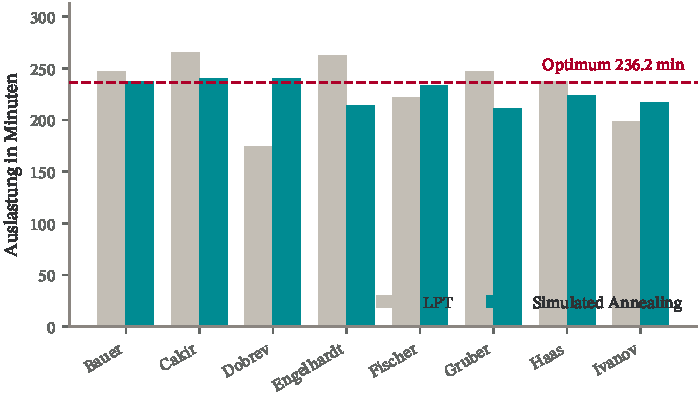
\includegraphics[alt={Gruppiertes Balkendiagramm: Auslastung in Minuten je Mitarbeiterin und Mitarbeiter, jeweils für die LPT-Startlösung und nach Simulated Annealing, dazu eine gestrichelte Linie beim Optimum. Nach Simulated Annealing liegen die Balken gleichmäßiger um das Optimum.}]{Abbildungen/auslastung.pdf}
  \caption[Auslastung je Mitarbeiter]{Auslastung der Mitarbeitenden bei
    der \acs{lpt}-Startlösung und nach dem Verfahren. Der Makespan ist
    die Höhe des jeweils höchsten Balkens.}
  \label{abb:auslastung}
\end{figure}

Auffällig ist, dass selbst die optimale Lösung kein waagerechtes Profil
erzeugt. Die Auslastungen streuen weiterhin um einige Minuten. Das ist
keine Schwäche des Lösers, sondern eine Eigenschaft des Problems:
Aufgaben sind unteilbar, und die Qualifikationen schränken ein, wer was
übernehmen darf. Eine vollkommen gleichmäßige Verteilung ist im
Allgemeinen unzulässig. Sie ist genau die Annahme, auf der die triviale
untere Schranke von \UntereSchranke{} Minuten beruht -- und deshalb
liegt das wahre Optimum mit \Optimum{} Minuten um \LueckeSchranke{}
Prozent darüber.

Wohin die Arbeitszeit fließt, zeigt Abbildung~\ref{abb:sankey}. Die
Bandbreite entspricht den Minuten, die von einer Qualifikation auf einen
Mitarbeitenden entfallen. Sichtbar wird, dass sich die Last der seltenen
Qualifikationen auf wenige Personen konzentriert: Wer als Einziger
schweißen kann, bekommt die Schweißarbeit, unabhängig davon, wie
ausgelastet er ohnehin ist.

\begin{figure}[tb]
  \centering
  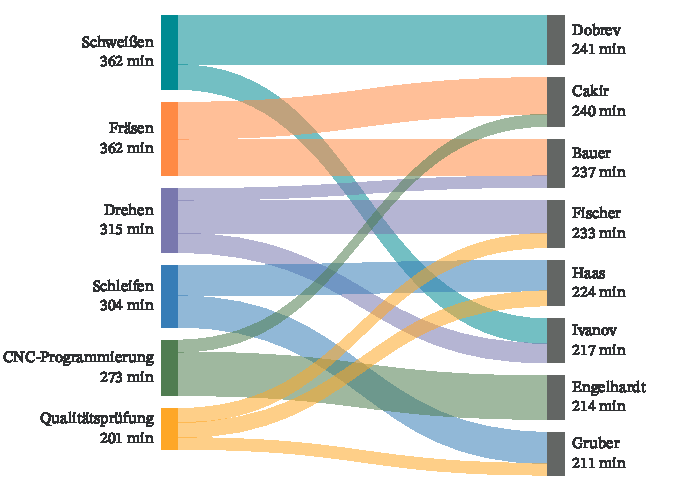
\includegraphics[alt={Flussdiagramm: Bänder führen von den Qualifikationen links zu den Mitarbeitenden rechts; die Breite eines Bandes entspricht den zugeordneten Minuten.}]{Abbildungen/sankey.pdf}
  \caption[Fluss der Arbeitszeit]{Fluss der Arbeitszeit von den
    Qualifikationen zu den Mitarbeitenden in der gefundenen Lösung. Die
    Bandbreite entspricht den Minuten.}
  \label{abb:sankey}
\end{figure}

\section{Wirkung der geglätteten Energie}
\label{sec:energiewirkung}

Abschnitt~\ref{sec:plateau} hat die geglättete Energie mit dem
Plateauproblem begründet. Ob das Argument trägt, ist eine empirische
Frage. Abbildung~\ref{abb:energien} beantwortet sie über je 20~Läufe
beider Varianten.

\begin{figure}[tb]
  \centering
  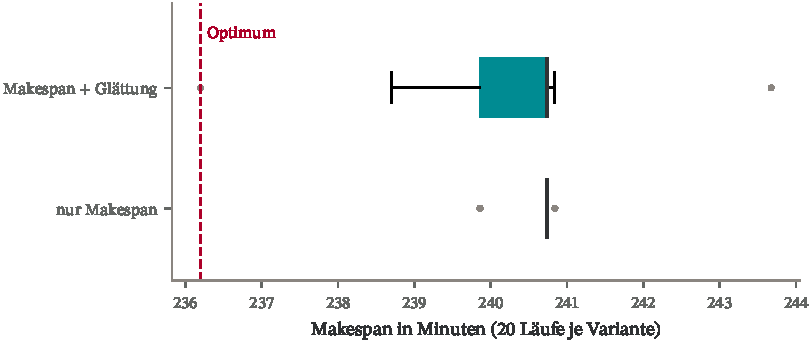
\includegraphics[alt={Kastendiagramme des Makespans über mehrere Läufe für zwei Energiefunktionen, dazu eine gestrichelte Linie beim Optimum. Nur mit Glättungsterm erreicht ein Lauf das Optimum.}]{Abbildungen/energien.pdf}
  \caption[Wirkung der geglätteten Energie]{Streuung des Makespans über
    je 20 Läufe. Mit der rohen Zielgröße als Energie erreicht kein Lauf
    das Optimum; mit dem Glättungsterm gelingt es.}
  \label{abb:energien}
\end{figure}

Der Befund ist deutlich. Mit der rohen Zielgröße liegen alle Läufe eng
beieinander bei \SaRohMittel{} Minuten im Mittel -- eng, aber
gleichmäßig zu hoch. Das Verfahren findet zuverlässig dasselbe lokale
Optimum und kommt nicht darüber hinaus. Mit dem Glättungsterm sinkt der
Mittelwert auf \SaMittel{} Minuten, und der beste Lauf erreicht mit
\SaBestes{} Minuten das Optimum.

Bemerkenswert ist der Preis: Die Streuung nimmt zu. Die geglättete
Variante ist im Mittel besser, aber weniger vorhersagbar. Wer einen
einzelnen Lauf betrachtet, kann schlechter abschneiden als mit der rohen
Variante. Das ist der übliche Handel zwischen Erkundung und
Verlässlichkeit und ein Argument dafür, mehrere Läufe zu rechnen und den
besten zu nehmen -- was bei einer Rechenzeit von \SaMillisekunden{}
Millisekunden je Lauf keine ernsthafte Hürde ist.

Abbildung~\ref{abb:konvergenz} zeigt einen einzelnen Lauf im Verlauf.
Die aktuelle Lösung schwankt anfangs stark -- die Temperatur lässt
Verschlechterungen zu --, und beruhigt sich mit sinkender Temperatur.
Die beste gefundene Lösung fällt in Stufen: lange Phasen ohne
Fortschritt, unterbrochen von Sprüngen. Genau dieses Muster erwartet man
bei einer plateaulastigen Zielgröße.

\begin{figure}[tb]
  \centering
  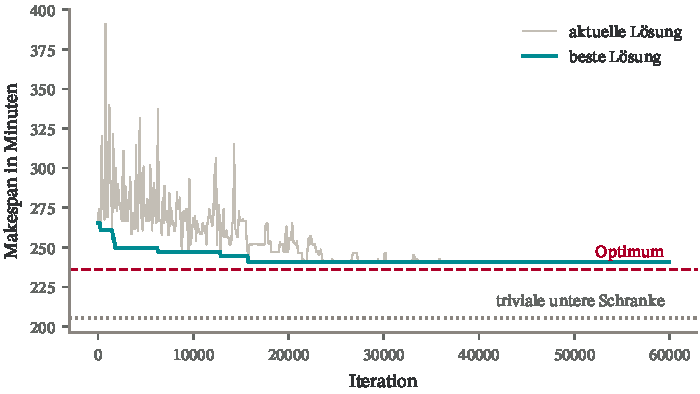
\includegraphics[alt={Liniendiagramm über die Iterationen: aktuelle und beste Lösung fallen ab und nähern sich der Linie des Optimums; darunter die untere Schranke.}]{Abbildungen/konvergenz.pdf}
  \caption[Verlauf eines Laufs]{Verlauf eines einzelnen Laufs: aktuelle
    und beste Lösung, dazu Optimum und triviale untere Schranke.}
  \label{abb:konvergenz}
\end{figure}

\section{Vergleich der Verfahren}
\label{sec:vergleich}

Tabelle~\ref{tab:verfahren} auf Seite~\pageref{tab:verfahren} hat die
Verfahren bereits gegenübergestellt. Die Rangfolge ist eindeutig: Die
bisherige Praxis entspricht ungefähr der Greedy-Regel mit
\MakespanGreedy{} Minuten, \ac{lpt} verbessert das auf \MakespanLPT{}
Minuten, \ac{sa} auf \MakespanSA{} Minuten, und das exakte Verfahren
erreicht \Optimum{} Minuten.

Gegenüber der heutigen Praxis spart die optimale Lösung rund eine halbe
Stunde je Fertigungslos. Das ist der Ertrag, um den es geht, und er ist
mit einem Standardlöser in weniger als einer Sekunde zu haben.

Damit stellt sich die Frage nach dem Sinn der Heuristik in aller
Schärfe. Auf dieser Instanz ist \ac{sa} in jeder Hinsicht unterlegen: Es
braucht mehr Rechenzeit als der exakte Löser, findet ein um
\AbstandSA{} Prozent schlechteres Ergebnis und gibt keinerlei Garantie.
Wer nur diese Instanz betrachtet, sollte den Löser nehmen.

\section{Verhalten bei wachsender Instanz}
\label{sec:skalierung}

Der Vorteil des exakten Verfahrens ist allerdings an die Größe gebunden.
Um zu prüfen, wo die Grenze liegt, wurden Zufallsinstanzen derselben
Struktur mit wachsender Zahl von Arbeitsgängen erzeugt und beide
Verfahren darauf angewendet. Dem Löser wurde eine Zeitschranke von
30~Sekunden gesetzt.

\begin{table}[tb]
  \centering
  % Automatisch erzeugt von Code/tabellen.py -- nicht von Hand ändern.
% Quelle: Code/daten.py und Ergebnisse/*.json

\begin{tabular}{@{}S[table-format=3.0]S[table-format=2.0]S[table-format=3.2]S[table-format=2.1]lS[table-format=3.2]S[table-format=1.1]S[table-format=+1.2]@{}}
\toprule
& & \multicolumn{3}{c}{MILP (GLPK)} & \multicolumn{2}{c}{Simulated Annealing} & \\
\cmidrule(lr){3-5}\cmidrule(lr){6-7}
{Aufg.} & {Mitarb.} & {Makespan} & {Zeit} & {Status} & {Makespan} & {Zeit} & {Abstand} \\
& & {min} & {s} & & {min} & {s} & {\%} \\
\midrule
  24 & 8 & 276.77 & 1.1 & optimal & 280.80 & 0.3 & +1.46 \\
  40 & 10 & 381.45 & 0.0 & optimal & 381.45 & 0.4 & +0.00 \\
  60 & 12 & 529.71 & 30.0 & Zeitschranke & 529.33 & 0.5 & -0.07 \\
  80 & 14 & 489.17 & 30.0 & Zeitschranke & 484.03 & 0.7 & -1.05 \\
  120 & 18 & 707.27 & 30.0 & Zeitschranke & 707.27 & 1.0 & +0.00 \\
\bottomrule
\end{tabular}

  \caption[Verhalten bei wachsender Instanz]{Beide Verfahren auf
    Zufallsinstanzen wachsender Größe. Ein negativer Abstand bedeutet,
    dass Simulated Annealing die beste Lösung schlägt, die der Löser
    innerhalb der Zeitschranke gefunden hat.}
  \label{tab:skalierung}
\end{table}

\begin{figure}[tb]
  \centering
  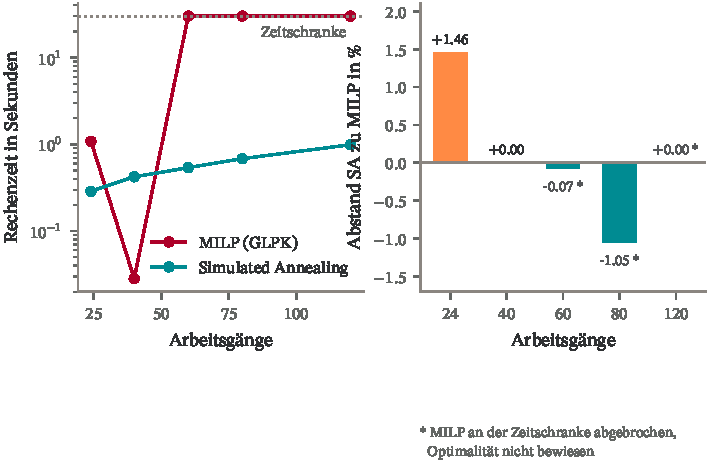
\includegraphics[alt={Links: Rechenzeit von MILP und Simulated Annealing über der Zahl der Arbeitsgänge, logarithmisch; das MILP stößt ab mittlerer Größe an die Zeitschranke. Rechts: Balken mit dem prozentualen Abstand von Simulated Annealing zum MILP je Instanzgröße.}]{Abbildungen/skalierung.pdf}
  \caption[Rechenzeit und Güte über die Instanzgröße]{Rechenzeit
    (links, logarithmisch) und Abstand der Lösungen (rechts) über die
    Zahl der Arbeitsgänge.}
  \label{abb:skalierung}
\end{figure}

Tabelle~\ref{tab:skalierung} und Abbildung~\ref{abb:skalierung} zeigen
den Umschlag. Bis 40~Arbeitsgänge löst \ac{glpk} beweisbar optimal,
teilweise in Sekundenbruchteilen. Ab 60~Arbeitsgängen läuft der Löser in
die Zeitschranke und kann die Optimalität nicht mehr belegen. Von da an
liefert \ac{sa} in unter einer Sekunde Lösungen, die gleich gut oder
besser sind als das, was der Löser in 30~Sekunden erreicht -- bei
80~Arbeitsgängen um gut ein Prozent besser.

Zwei Beobachtungen verdienen Beachtung. Erstens verläuft die Rechenzeit
des Lösers nicht monoton: Die Instanz mit 40~Arbeitsgängen ist leichter
als die mit 24. Die Schwierigkeit einer Instanz hängt eben nicht allein
an ihrer Größe, sondern an ihrer Struktur -- eine bekannte, aber gern
übersehene Eigenschaft ganzzahliger Probleme. Zweitens wächst die
Rechenzeit von \ac{sa} nur schwach, weil sie durch die feste Zahl von
Iterationen bestimmt ist und nicht durch die Instanz. Das macht sie
planbar, sagt aber nichts über die Güte.

\section{Grenzen der Aussage}

Die Ergebnisse dieses Kapitels gelten für die untersuchte Instanz und
die untersuchten Zufallsinstanzen. Fünf Größen mit je einer Instanz sind
eine schmale Grundlage; belastbar wäre eine Auswertung über mehrere
Instanzen je Größe mit Angabe der Streuung. Ebenso wurde nur ein Löser
betrachtet. Kommerzielle Löser sind auf ganzzahligen Problemen
regelmäßig um Größenordnungen schneller als \ac{glpk}, was den
Umschlagpunkt nach oben verschieben dürfte -- vermutlich deutlich.

Die Aussage \enquote{ab etwa 60~Arbeitsgängen lohnt sich die Heuristik}
ist deshalb genauer zu lesen als: \enquote{mit diesem Löser, dieser
Zeitschranke und dieser Instanzstruktur}. Die Struktur des Arguments
bleibt gültig, die Zahl ist keine Konstante.

\chapter{Zusammenfassung und Ausblick}
\label{kap:zusammenfassung}

\section{Zusammenfassung}

Diese Arbeit hat die Verteilung von Arbeitsgängen auf Mitarbeitende bei
Erpolino als Optimierungsproblem formuliert und zwei Wege verglichen,
es zu lösen.

Das Problem ließ sich als ganzzahliges lineares Programm formulieren, in
der Notation des Scheduling als $R\,|\,M_j\,|\,C_{\max}$. Für das
betrachtete Fertigungslos aus \ZahlAufgaben{} Arbeitsgängen und
\ZahlMitarbeiter{} Mitarbeitenden liefert \ac{glpk} in \MilpSekunden{}
Sekunden eine beweisbar optimale Gesamtdauer von \Optimum{} Minuten.
Gegenüber der bisherigen Praxis, die ungefähr einer Greedy-Regel
entspricht und \MakespanGreedy{} Minuten benötigt, ist das eine
Ersparnis von rund einer halben Stunde je Los.

Die Forschungsfrage lässt sich damit beantworten: Ja, die Verteilung
lässt sich sinnvoll optimieren, und der Ertrag ist messbar. Der
überraschende Teil der Antwort betrifft das Wie.

\section{Stärken und Schwächen der Verfahren}

\subsection{Das exakte Verfahren}

Seine Stärke ist die \Index{Gütegarantie}. Der Löser liefert nicht nur
eine Lösung, sondern den Beweis, dass es keine bessere gibt. Diese
Aussage kann keine Heuristik machen, und sie ist in der Diskussion mit
der Arbeitsvorbereitung viel wert: Sie beendet die Frage, ob nicht doch
noch etwas herauszuholen wäre.

Hinzu kommt die Beschreibbarkeit. Das Modell in
Anhang~\ref{anh:mathprog} umfasst rund 20 Zeilen und ist ohne
Programmierkenntnisse lesbar. Ändert sich eine Anforderung, ändert sich
eine Nebenbedingung -- nicht ein Algorithmus.

Seine Schwäche ist das Laufzeitverhalten. Es ist im schlechtesten Fall
exponentiell, und Abschnitt~\ref{sec:skalierung} zeigt, dass der
schlechteste Fall nicht theoretisch bleibt: Ab 60~Arbeitsgängen erreicht
\ac{glpk} die Zeitschranke, ohne die Optimalität zu belegen. Zudem ist
die Rechenzeit nicht vorhersagbar -- die Instanz mit 40~Arbeitsgängen
war leichter als die mit 24.

\subsection{Simulated Annealing}

Seine Stärke ist die planbare Rechenzeit. Sie hängt an der Zahl der
Iterationen, nicht an der Instanz, und wächst über den untersuchten
Bereich nur schwach. Wo der Löser aufgibt, liefert das Verfahren
weiterhin brauchbare Lösungen, bei 80~Arbeitsgängen sogar bessere als
der Löser in 30~Sekunden.

Seine Schwächen sind gravierender, als es die Zahlen nahelegen. Es gibt
keine Gütegarantie: Ohne Vergleichswert bleibt unbekannt, wie weit eine
Lösung vom Optimum entfernt ist. Genau dieser Vergleichswert fehlt aber
in dem Bereich, in dem das Verfahren gebraucht wird -- dort, wo der
Löser versagt. Das ist kein Detail, sondern die eigentliche Schwäche der
Methode.

Hinzu kommt die Empfindlichkeit gegenüber Entscheidungen, die nicht aus
dem Problem folgen. Abschnitt~\ref{sec:energiewirkung} hat gezeigt, dass
die Wahl der Energie über Erfolg und Misserfolg entscheidet: Mit der
naheliegenden rohen Zielgröße erreicht kein einziger Lauf das Optimum,
mit dem Glättungsterm gelingt es. Abkühlplan, Nachbarschaft und
Iterationszahl wirken ähnlich. Nichts davon steht im Modell; alles davon
muss erprobt werden.

\subsection{Empfehlung}

Für Erpolino in der heutigen Größenordnung lautet die Empfehlung
eindeutig: das exakte Verfahren. Es ist schneller, besser und liefert
eine Garantie. Die Heuristik ist die aufwendigere Lösung des leichteren
Problems.

Das ist ein negatives Ergebnis für den Hauptteil dieser Arbeit, und es
ist keines, das sich verstecken lässt. Es ist zugleich das nützlichste
Ergebnis: Ein Unternehmen, das die Zuordnung verbessern will, sollte
nicht mit einer Metaheuristik beginnen. Es sollte mit einem Modell
beginnen.

Die Heuristik wird interessant, sobald die Instanz wächst -- durch mehr
Arbeitsgänge, weitere Standorte oder einen längeren Planungshorizont.
Der gemessene Umschlag bei etwa 60~Arbeitsgängen gilt für \ac{glpk}; mit
einem kommerziellen Löser dürfte er deutlich später liegen.

\section{Ausblick}

Drei Richtungen bieten sich an.

\emph{Das Modell erweitern.} Die Annahmen aus
Abschnitt~\ref{sec:annahmen} sind spürbare Vereinfachungen.
\Index{Rüstzeiten}, Reihenfolgeabhängigkeiten und Fälligkeitstermine
fehlen. Termine ließen sich als Nebenbedingung ergänzen, ohne die
Struktur zu ändern; Reihenfolgeabhängigkeiten führen dagegen auf ein
anderes Problem -- ein Job-Shop --, das erheblich schwerer ist
\parencite{pinedo2016scheduling}.

\emph{Die Zielgröße hinterfragen.} Der Makespan behandelt alle Aufgaben
gleich. In der Praxis sind manche Aufträge dringender als andere. Eine
gewichtete Zielgröße oder die Summe der Verspätungen wäre näher an dem,
was die Arbeitsvorbereitung tatsächlich abwägt.

\emph{Die Datengrundlage verbreitern.} Die Effizienzwerte der
Qualifikationsmatrix stammen aus Erfahrungswerten. Ob sie stimmen, ist
offen, und das Ergebnis hängt unmittelbar an ihnen. Aus dem
\ac{erp}-System ließen sich Ist-Zeiten gewinnen und die Matrix
empirisch schätzen. Ohne diesen Schritt optimiert das Verfahren
zuverlässig auf Zahlen, deren Herkunft niemand belegen kann -- und das
ist am Ende das größere Risiko als die Wahl des Verfahrens.


%%%%%%%%%%%%%%%%%%%%%%%%%%%%%%%%%%%%%%%%%%%%%%%%%%%%%%%%%%%%%%%%%%%%%%%
\printbibliography[heading=bibintoc]

%%%%%%%%%%%%%%%%%%%%%%%%%%%%%%%%%%%%%%%%%%%%%%%%%%%%%%%%%%%%%%%%%%%%%%%
\appendix

\chapter{Quelltext des Verfahrens}
\label{anh:quelltext}

Der vollständige Quelltext liegt dem \Index{ergänzenden Material} bei.
Wiedergegeben ist hier der Kern des Verfahrens.

\lstinputlisting[
  language = Python,
  caption  = {Nachbarschaft und Abkühlung des Verfahrens (Auszug aus \texttt{Code/sa.py})},
  label    = {lst:sa},
  linerange= {nachbar-anfang-nachbar-ende},
]{Code/sa.py}

\chapter{Modell in MathProg}
\label{anh:mathprog}

\lstinputlisting[
  language = mathprog,
  caption  = {Das vollständige Modell in \Index{MathProg} (\texttt{Code/erpolino.mod})},
  label    = {lst:mod},
]{Code/erpolino.mod}

%%%%%%%%%%%%%%%%%%%%%%%%%%%%%%%%%%%%%%%%%%%%%%%%%%%%%%%%%%%%%%%%%%%%%%%
\printindex

%%%%%%%%%%%%%%%%%%%%%%%%%%%%%%%%%%%%%%%%%%%%%%%%%%%%%%%%%%%%%%%%%%%%%%%
% Die Richtlinie verlangt, erlaubt genutzte KI-Tools der Arbeit
% anzufügen; die Erklärung mit ki=kennzeichnung verweist darauf.
\addchap{Verwendete KI-Tools}

Für diese Arbeit wurden Werkzeuge der künstlichen Intelligenz zur
sprachlichen Überarbeitung einzelner Absätze eingesetzt. Modellbildung,
Implementierung, Auswertung und Bewertung der Ergebnisse stammen von der
Verfasserin beziehungsweise vom Verfasser.

% Die Erklärung ist der letzte Bestandteil der Arbeit. ki= ist Pflicht:
% keine, kennzeichnung oder ohnekennzeichnung (Richtlinie, Kapitel 7).
\eigenständigkeitserklärung[ki=kennzeichnung]
\end{document}
